Ths problem is a simulation to study the
amount of entrainment by thermal convection of a dense,
thin layer at the bottom of the model \cite{vaks97}. 
To the author's knowledge only two other publications \cite{taki03,vant07}
have presented results pertaining to this benchmark.
The results shown here after are obtained with my ELEFANT code using 
the particle-in-cell technique. 

The box is $2\times 1$, and contains two fluids:
\begin{center}
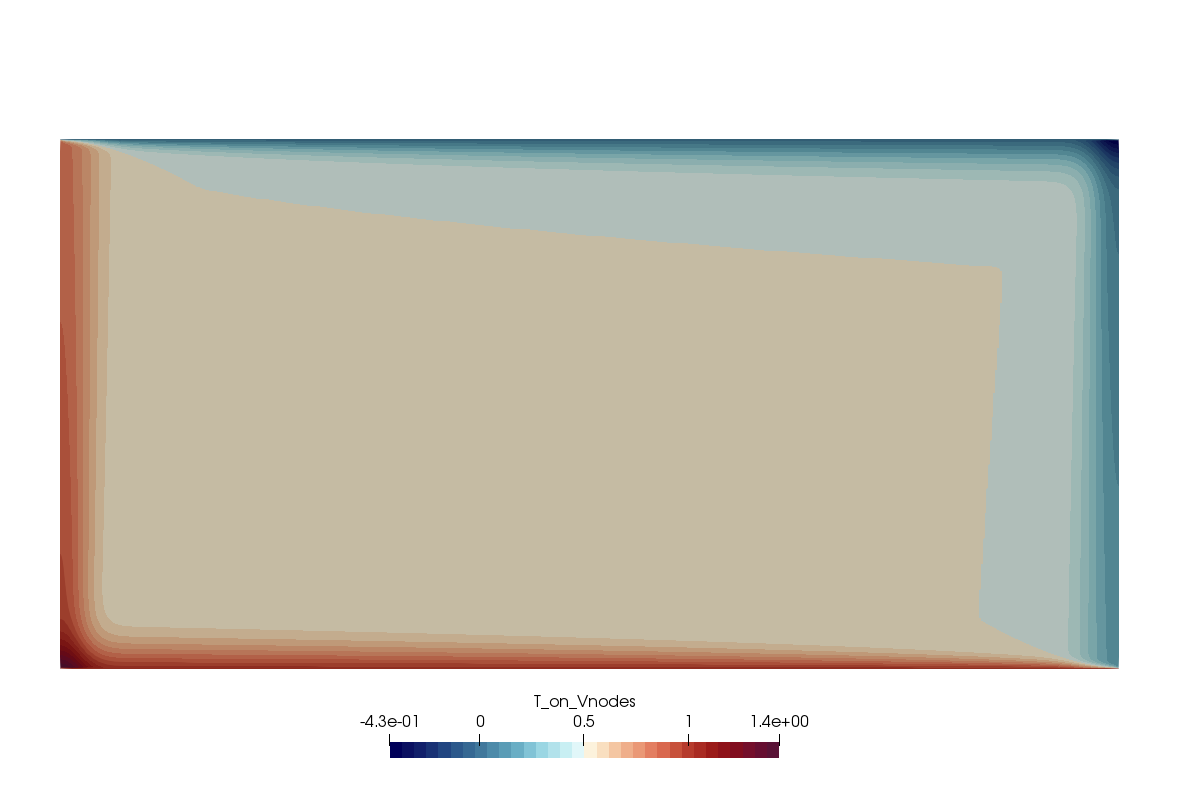
\includegraphics[width=0.45\linewidth]{images/benchmark_thinlayer/temperature_init}
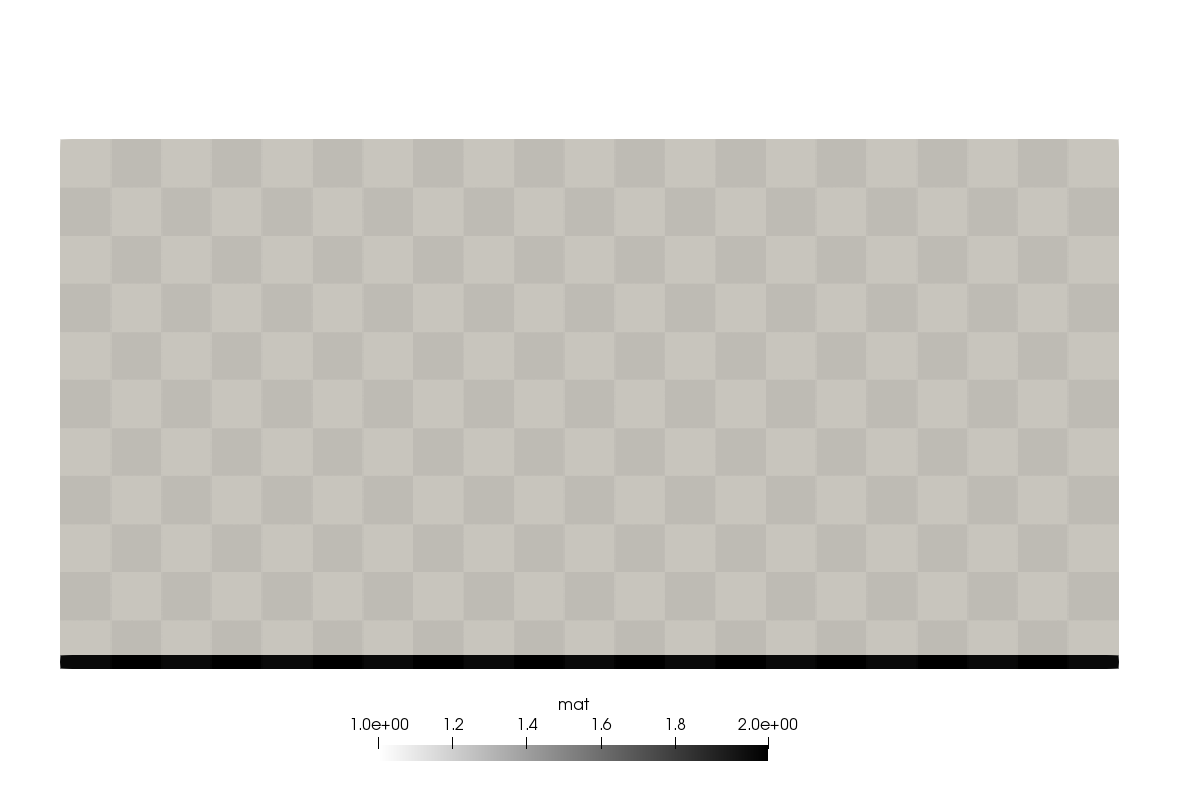
\includegraphics[width=0.45\linewidth]{images/benchmark_thinlayer/mat_init}
\end{center}
Fluid 1 has a density $\rho_1=1$ and a viscosity $\eta=1$.
Fluid 2 is heavier ($\rho_2=\rho_1 + \Delta \rho$) 
but has the same viscosity. 
Both fluids have a thermal expansion coefficient $\alpha=10^{-10}$, a 
thermal conductivity $k=1$, and a heat capacity coefficient $c_p=1$.
Fluid 2 is placed at the bottom of the box ($0\leq y \leq 0.025$).

This experiment is parameterised by the thermal Rayleigh number $Ra=300,000$ and 
and the compositional Rayleigh number $Ra_c=450,000$ which are defined as follows:

\begin{eqnarray}
Ra_T=\frac{\alpha \rho g \Delta T L_y^3}{\kappa \eta}
= \frac{\alpha \rho^2 g \Delta T L_y^3 c_p}{k \eta}
= \alpha g \\
Ra_c&=&\frac{ \Delta \rho g L_y^3}{\kappa \eta}
= \frac{ \rho \Delta \rho g L_y^3 c_p}{k \eta}
= \Delta \rho g
\end{eqnarray}
where I have used the relationship $\kappa=k/\rho c_p$.
$B$ is defined as $B=Ra_T/Ra_c$ so 
The gravity acceleration is therefore set to $g=Ra/\alpha$ and this yields $\Delta \rho=Ra_c/g=B Ra_T/g = B\times \alpha$.

Free-slip boundary conditions are imposed on all sides of the domain.
Temperature boundary conditions are $T(x,y=0)=1$ and 
$T(x,y=1)=0$. The analytical initial temperature field is given by 
\begin{equation}
T(x,y)=T_u(x,y)+T_l(x,y)+T_r(x,y)+T_s(x,y)-\frac{3}{2}
\end{equation}
where
\begin{eqnarray}
T_u(x,y) &=& \frac{1}{2} {\rm erf} \left(  \frac{1-y}{2} \sqrt{\frac{u_0}{x}} \right) \nonumber\\
T_l(x,y) &=& 1-\frac{1}{2} {\rm erf} \left( \frac{y}{2} \sqrt{\frac{u_0}{L_x-x}} \right) \nonumber\\
T_r(x,y) &=& \frac{1}{2} + \frac{Q}{2\sqrt{\pi}} \sqrt{\frac{u_0}{y+1}} \exp \left(  -\frac{x^2u_0}{4y+4} \right) \nonumber\\
T_s(x,y) &=& \frac{1}{2} - \frac{Q}{2\sqrt{\pi}} \sqrt{\frac{u_0}{2-y}} \exp \left(  -\frac{(L_x-x)^2u_0}{8-4y} \right) 
\end{eqnarray}
with
\begin{equation}
u_0=\frac{L_x^{7/3}}{(1+L_x^4)^{2/3}} \left(\frac{Ra}{2\sqrt{\pi}} \right)^{2/3}
\quad\quad
Q=2\sqrt{\frac{L_x}{\pi u_0}}
\end{equation}
Using $L_x=2$, $Ra=3\times10^5$, one gets
$u_0 \simeq 1469.315 $ and $Q\simeq 0.0416305$.

Given the small thickness of the bottom layer, it seems quite legitimate to 
investigate the influence of grid resolution on the simulation. 
I have therefore looked at the initial root mean square velocity measurement 
as a function of the element diagonal value (a proxy for the average resolution
in the case where elements are not square). 


Results are confirm that 
the element size plays a non negligible role at startup on the dynamics of the system.
Superimposed on the figure are the measurements provided by Prof. van Keken (black squares
in the gray box).
They agree well with my measurements but also indicate that 
none of the authors in the original study ran the experiment at a high-enough resolution
to start with (their results were therefore most likely resolution dependent).

We see that the number of markers per element at startup is critical at 
(very) low resolution but that it does not lead to 
significant velocity variations at high resolution. 

\begin{center}
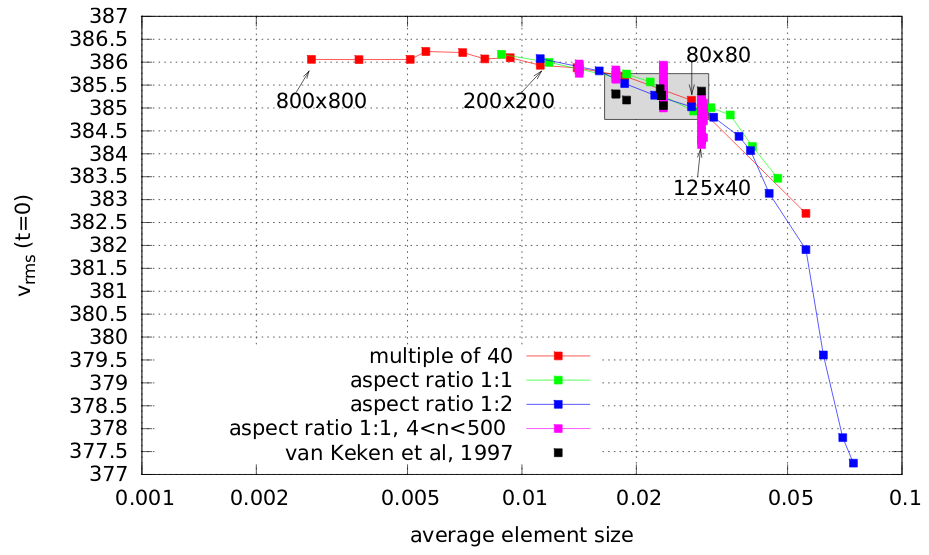
\includegraphics[width=0.65\linewidth]{images/benchmark_thinlayer/thie14}\\
{\scriptsize 
Thin layer entrainment experiment: root mean square velocity measurements at
$t=0$ as a function of the element diagonal size. 
The red square points correspond to resolutions where the number of elements in each direction 
is a multiple of 40 (i.e. $L_y/d$), so that no element would contain a mix of fluids 1 and 2. 
Pink points correspond to cases wherethe number of markers within each element was varied between 4 and 500 
(random spatial distribution). Taken from \cite{thie14}}
\end{center}


Looking at the root mean square velocity measurements, we see that
the measurements done with ELEFANT agree nicely with those presented in \cite{vaks97}. 
Past $t\sim0.015$, the curves diverge clearly across all codes and authors, 
so I only need to focus the comparison for times $t <0.015$. 
For the three tested resolutions,measurements agree well and fall within the grey curves 
representing all results of van Keken et al. 
Additional tests have been carried out concerning the value of the
Courant number (0.1 to 0.25) and the initial number of markers per element (100 or 200) 
and these parameters led to extremely similar results.

\begin{center}
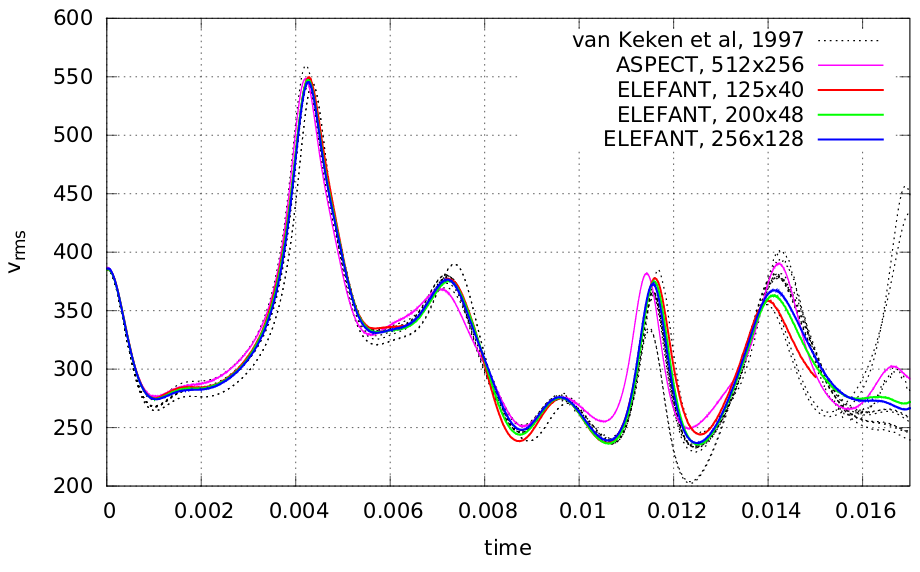
\includegraphics[width=0.65\linewidth]{images/benchmark_thinlayer/thie14b}\\
{\scriptsize Thin layer entrainment experiment. Root mean square velocity as a function of time.All results presented invan Keken et al.(1997) are collapsed in dashed lines. All simulationswere run with an initial marker density of 100 markers per element and with a Courant numberof 0.25. Taken from \cite{thie14}.}
\end{center}

As observed in van Keken et al., the dense layer is first swept 
into the lower left corner. Thermal instabilities then further develop in an asymmetrical way 
and entrain the dense material. Past $t\simeq 0.015$ the system becomes more 
and more chaotic with markers being randomly mixed in the system in a non-orderly fashion.

\begin{center}
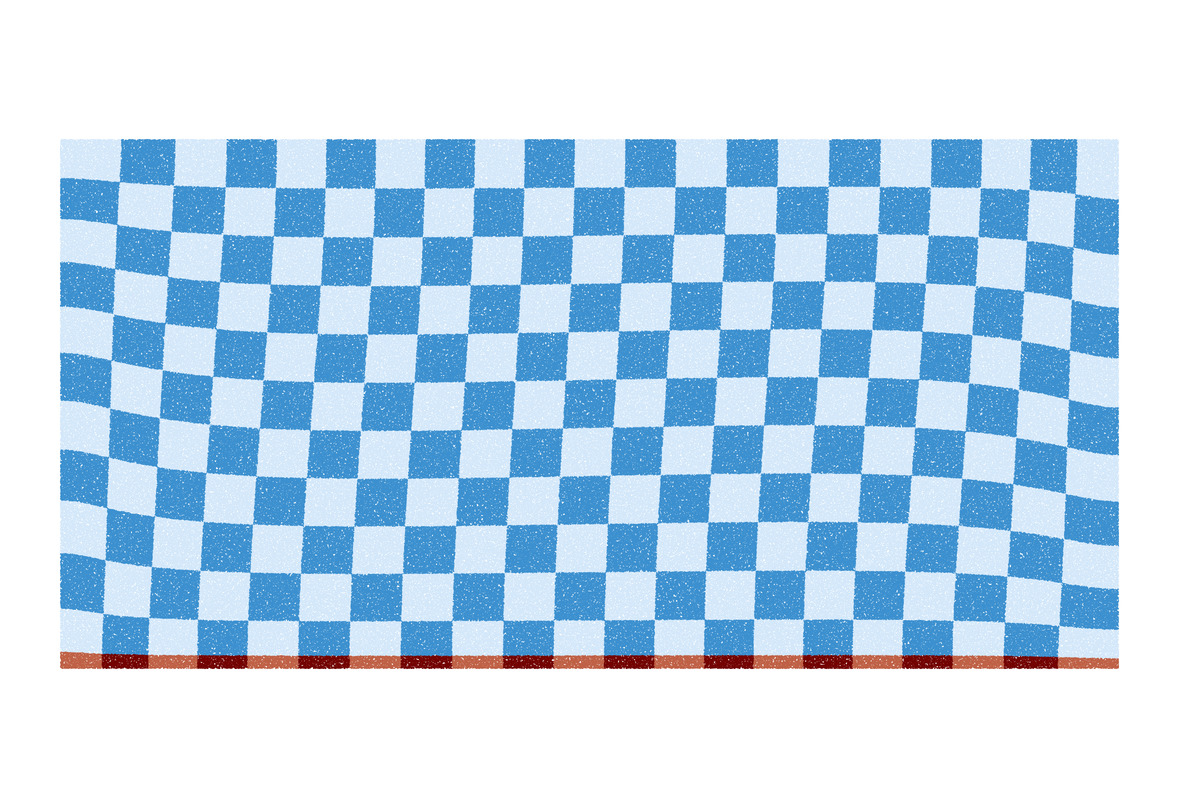
\includegraphics[width=0.23\linewidth]{images/benchmark_thinlayer/maarkers0000}
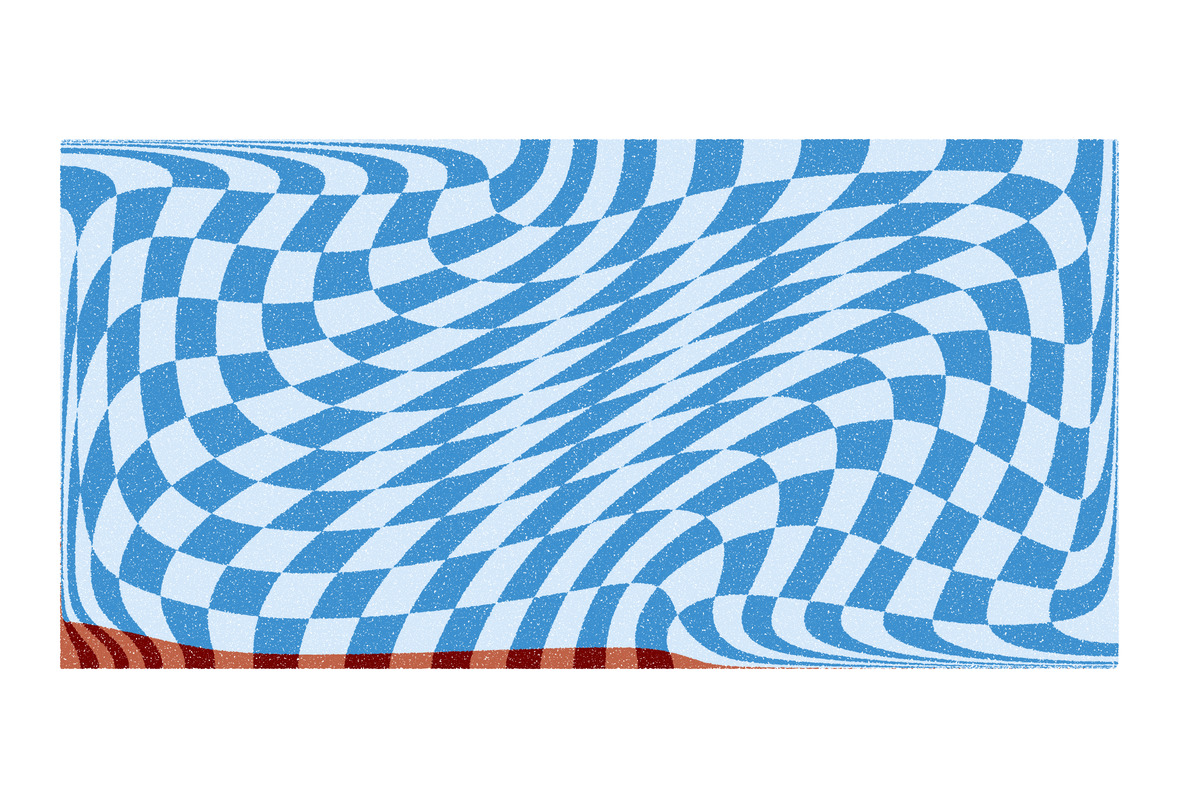
\includegraphics[width=0.23\linewidth]{images/benchmark_thinlayer/maarkers0025}
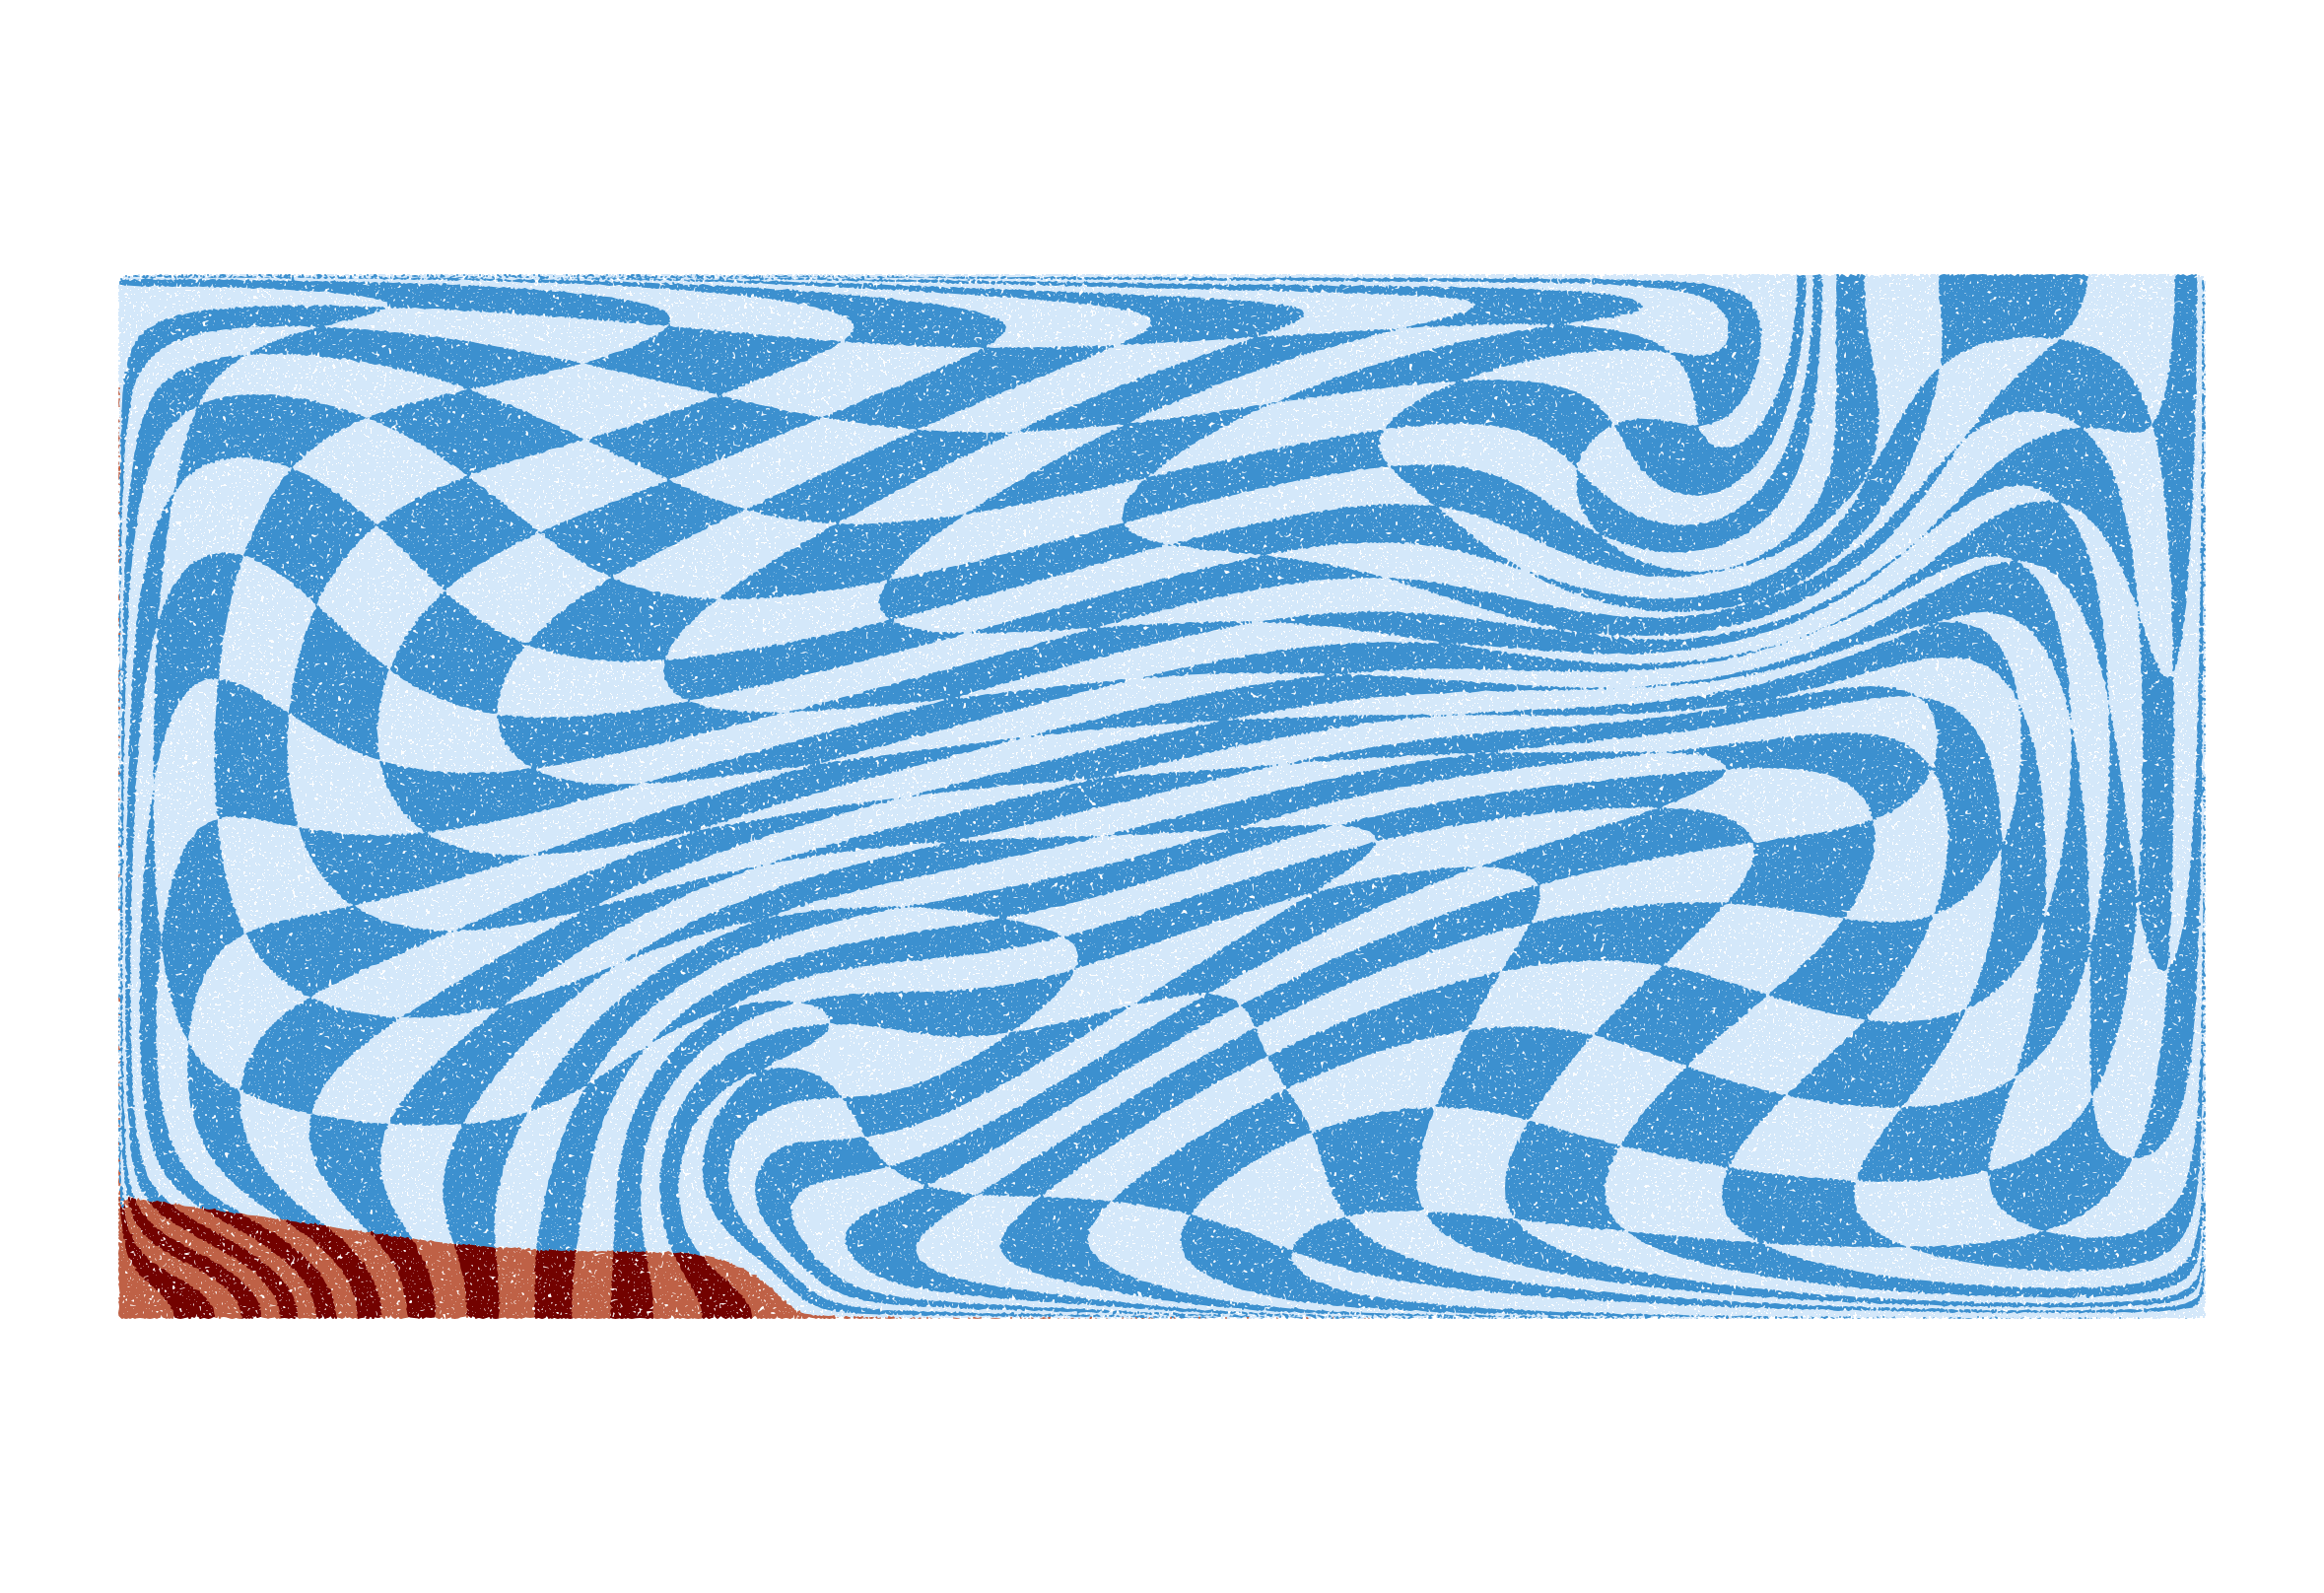
\includegraphics[width=0.23\linewidth]{images/benchmark_thinlayer/maarkers0050}
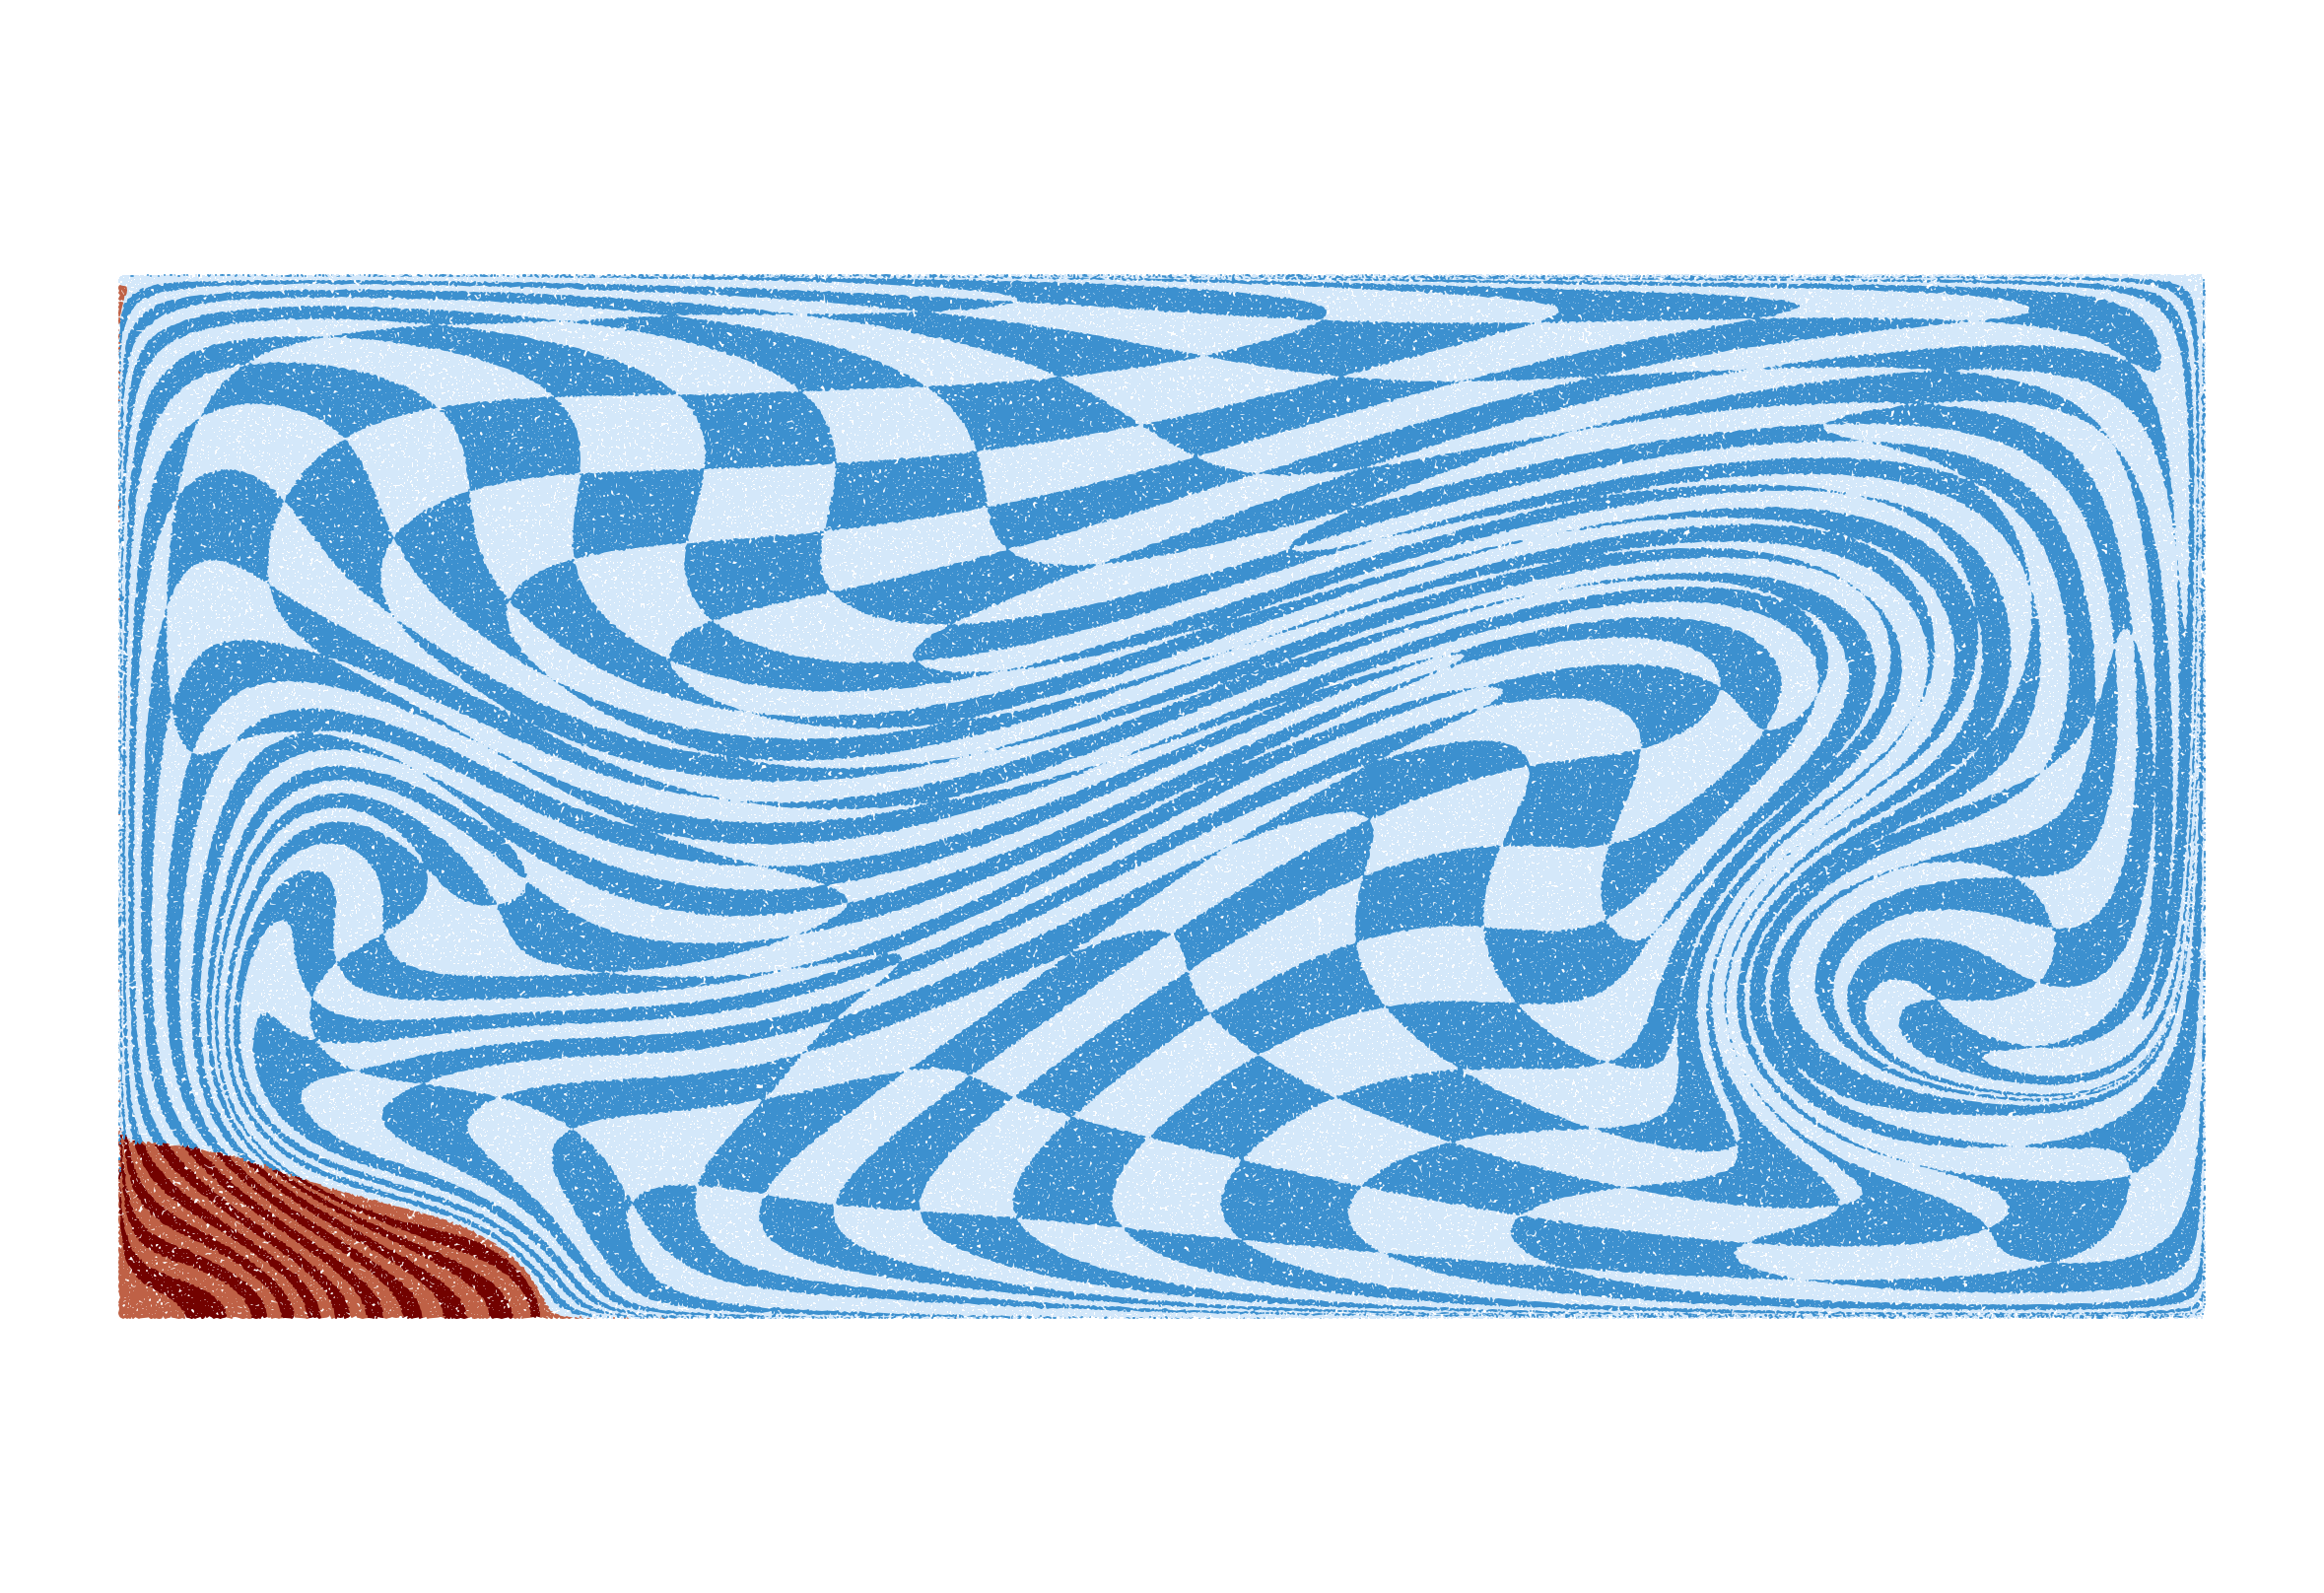
\includegraphics[width=0.23\linewidth]{images/benchmark_thinlayer/maarkers0075}\\
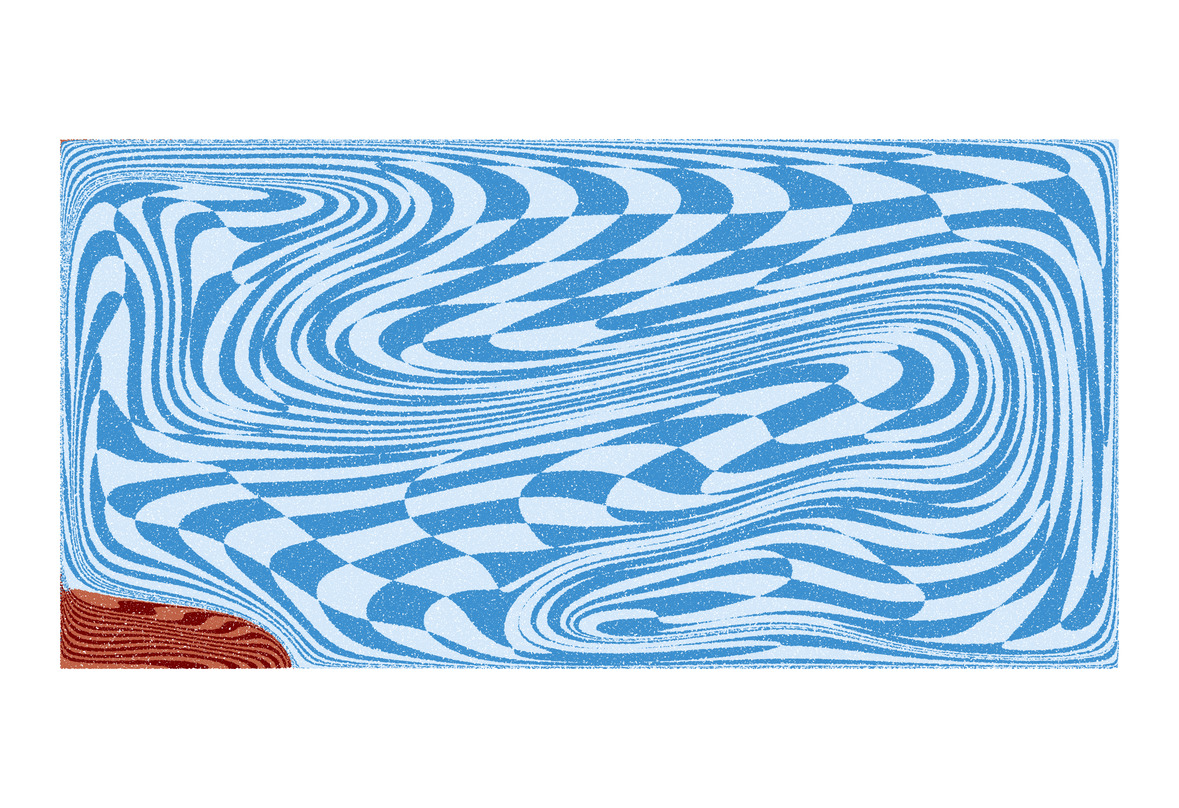
\includegraphics[width=0.23\linewidth]{images/benchmark_thinlayer/maarkers0100}
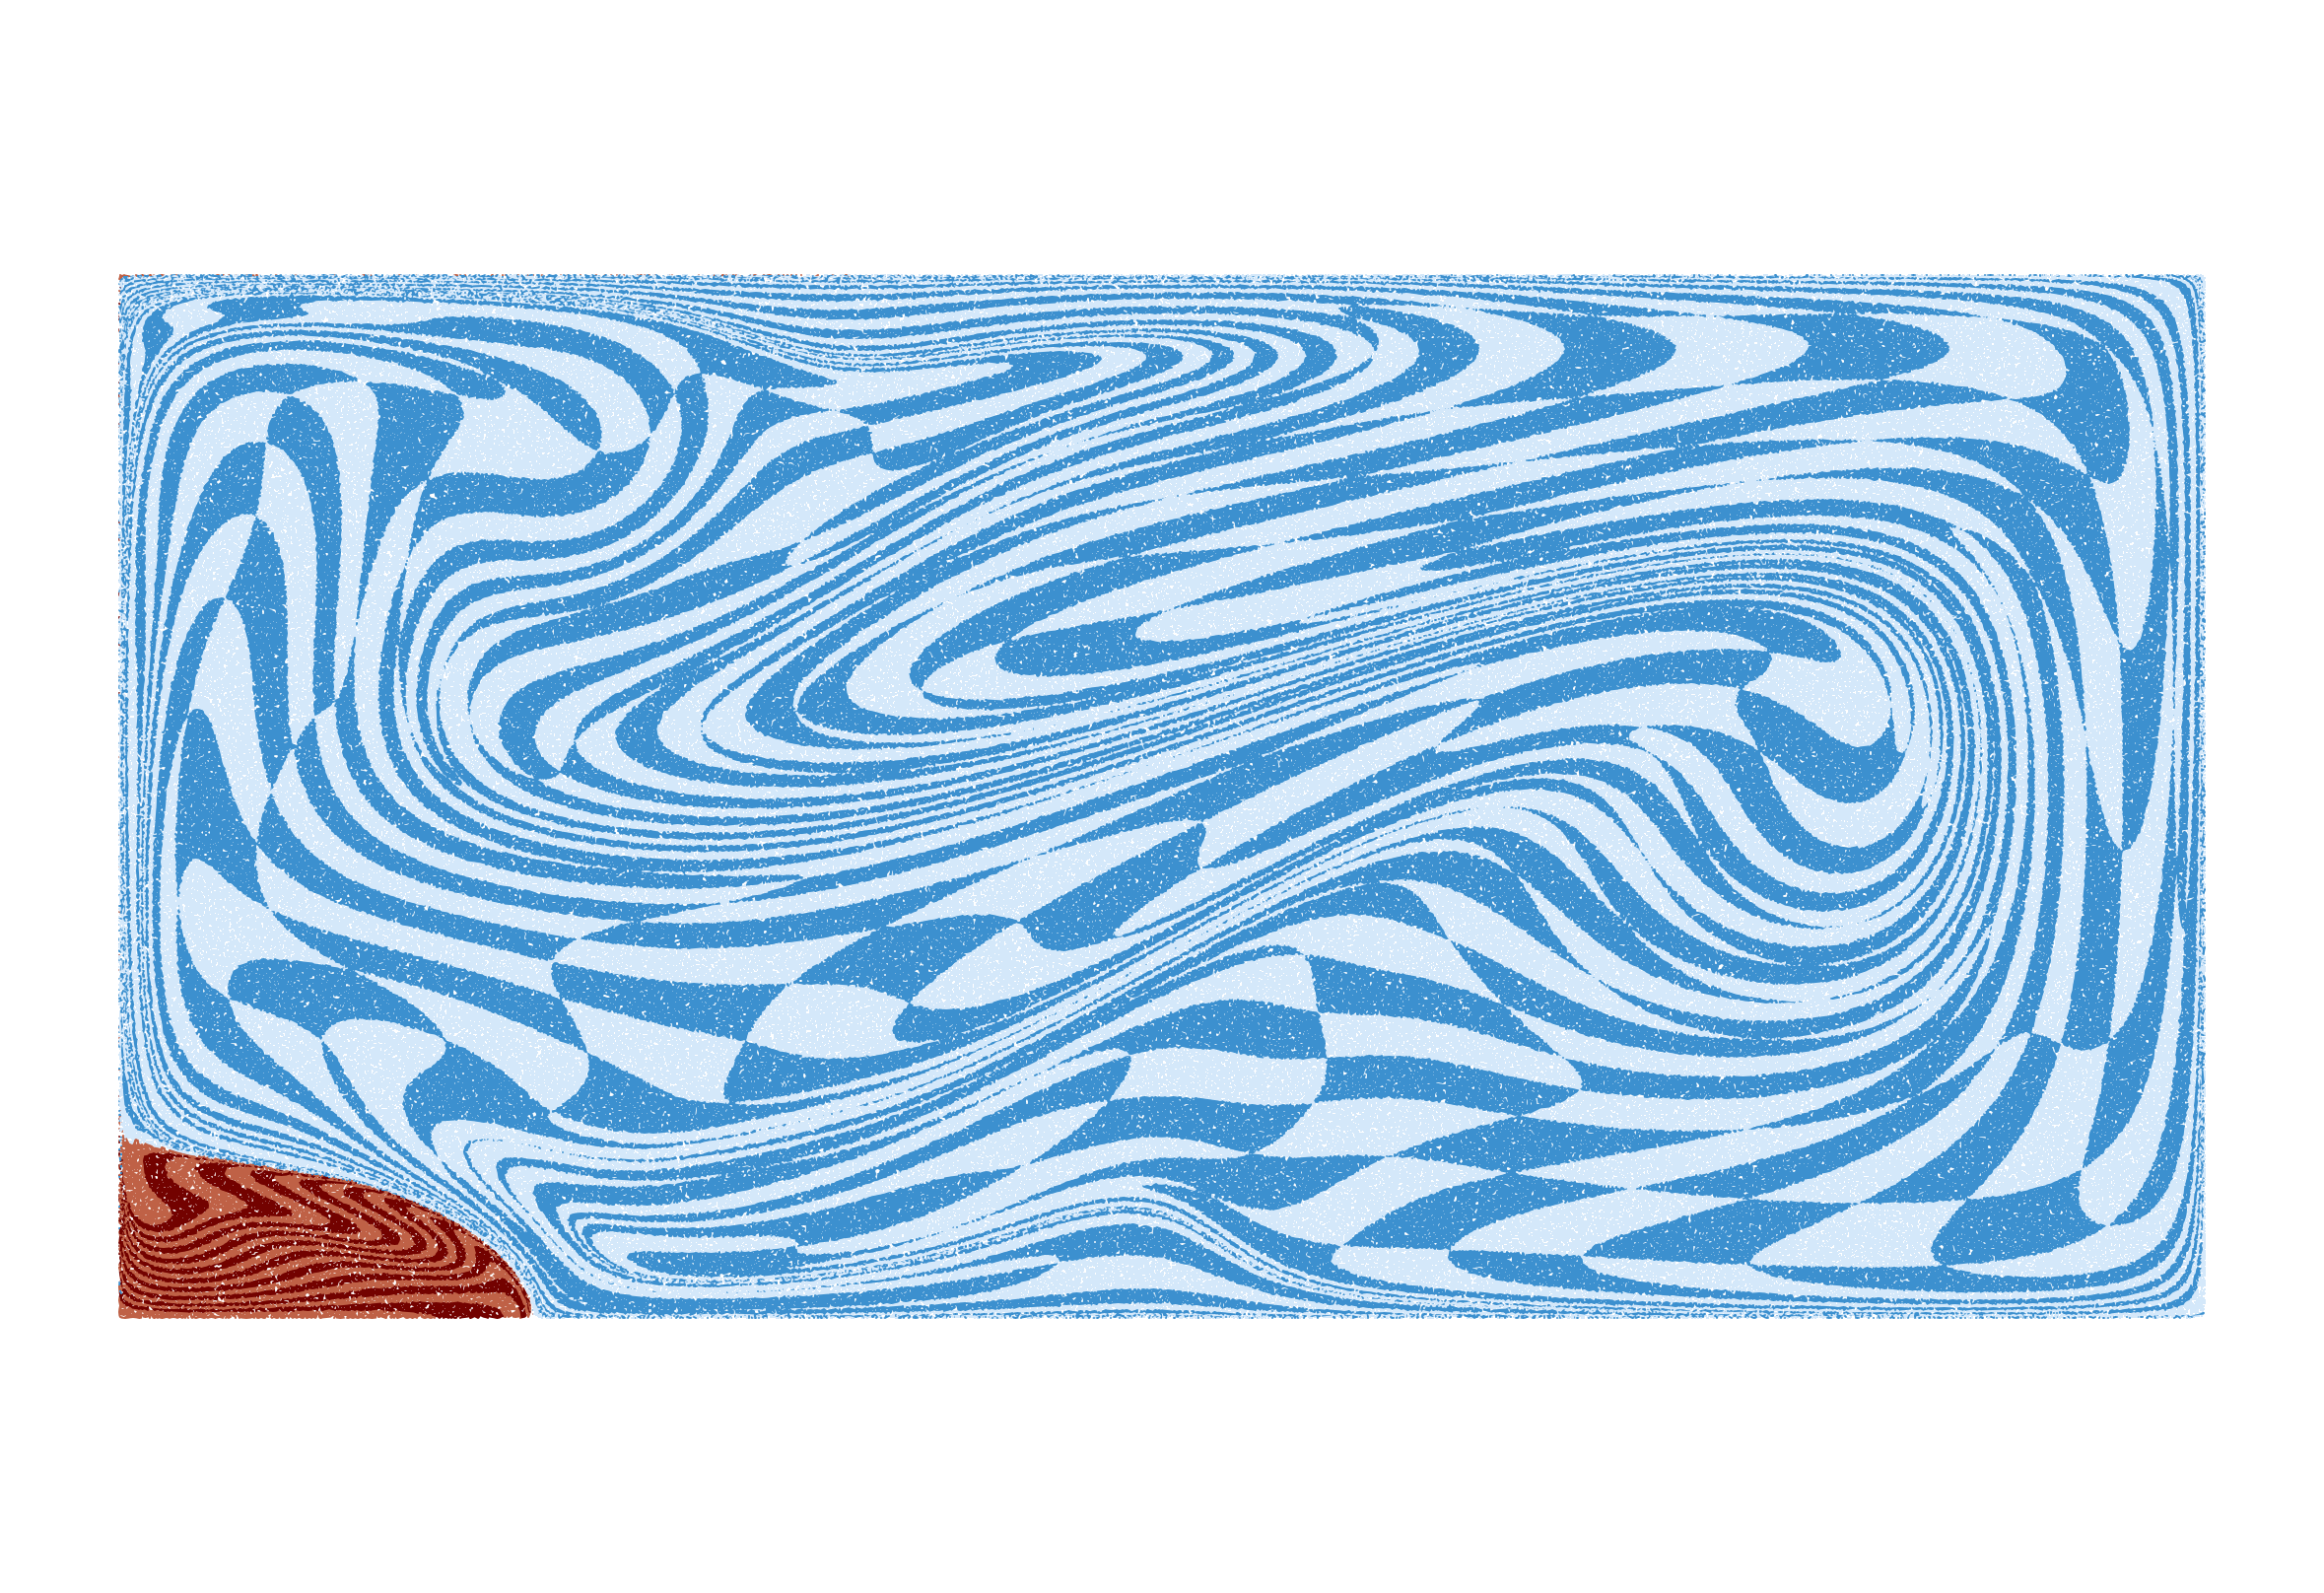
\includegraphics[width=0.23\linewidth]{images/benchmark_thinlayer/maarkers0125}
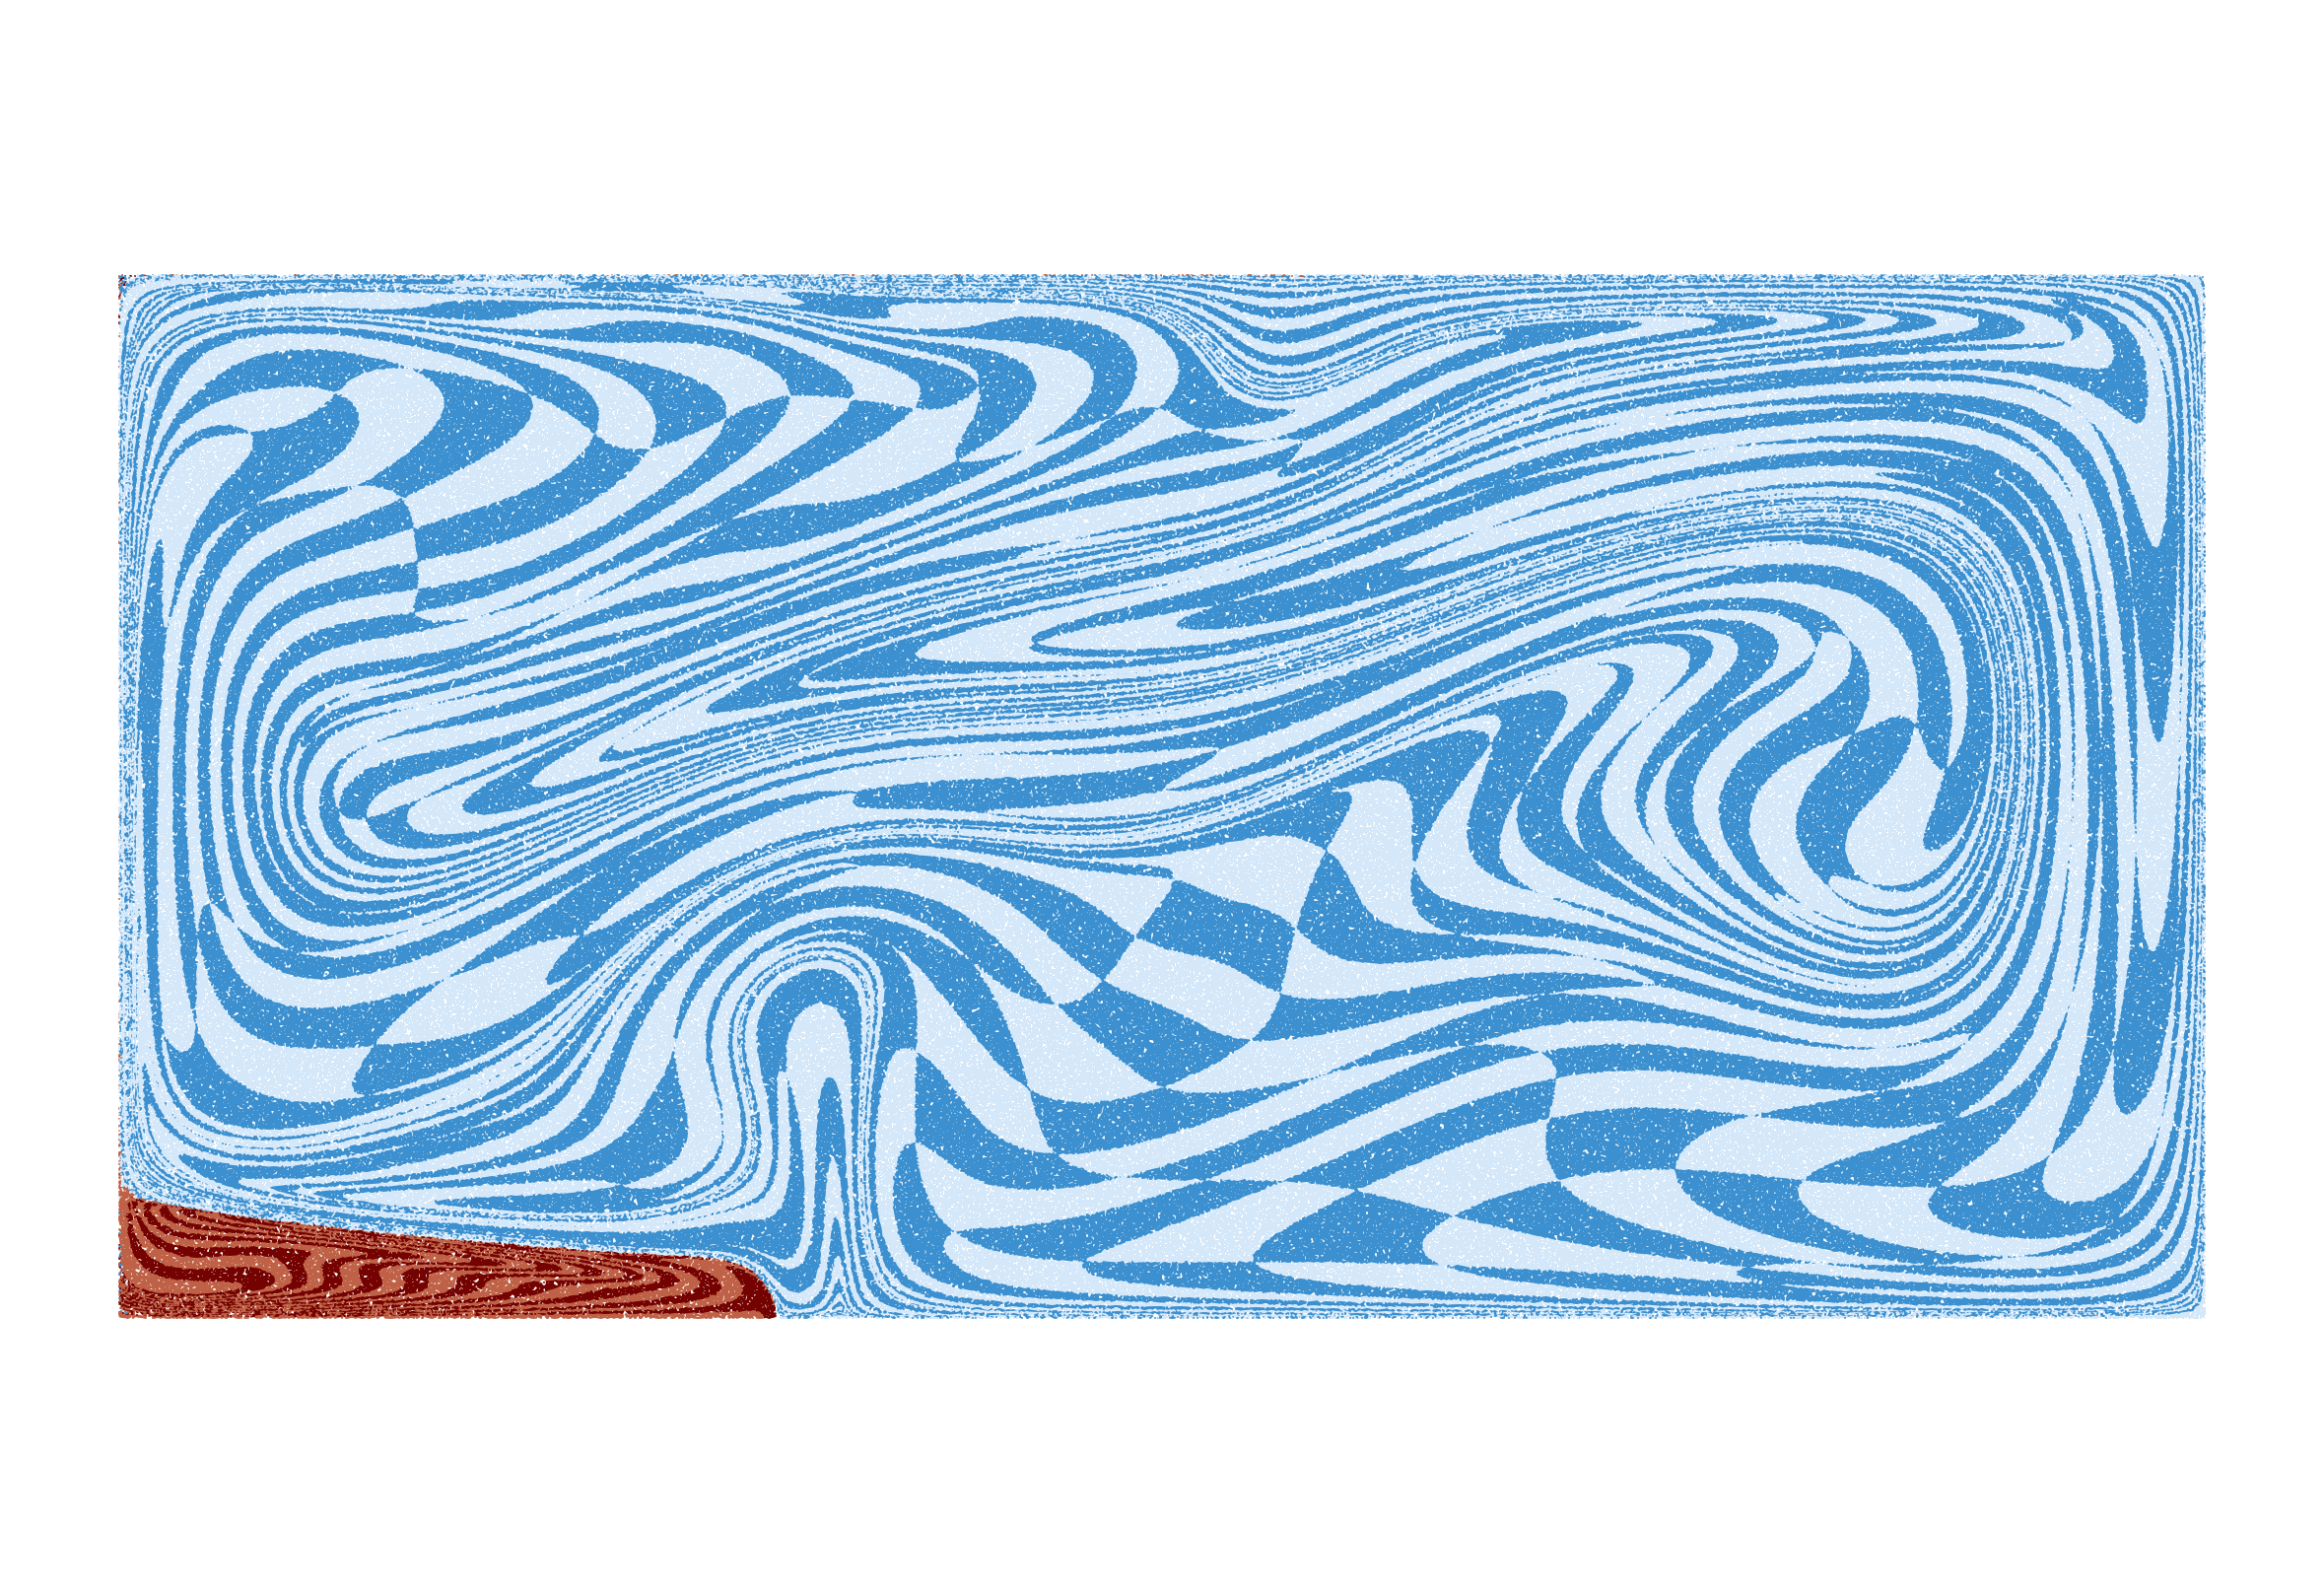
\includegraphics[width=0.23\linewidth]{images/benchmark_thinlayer/maarkers0150}
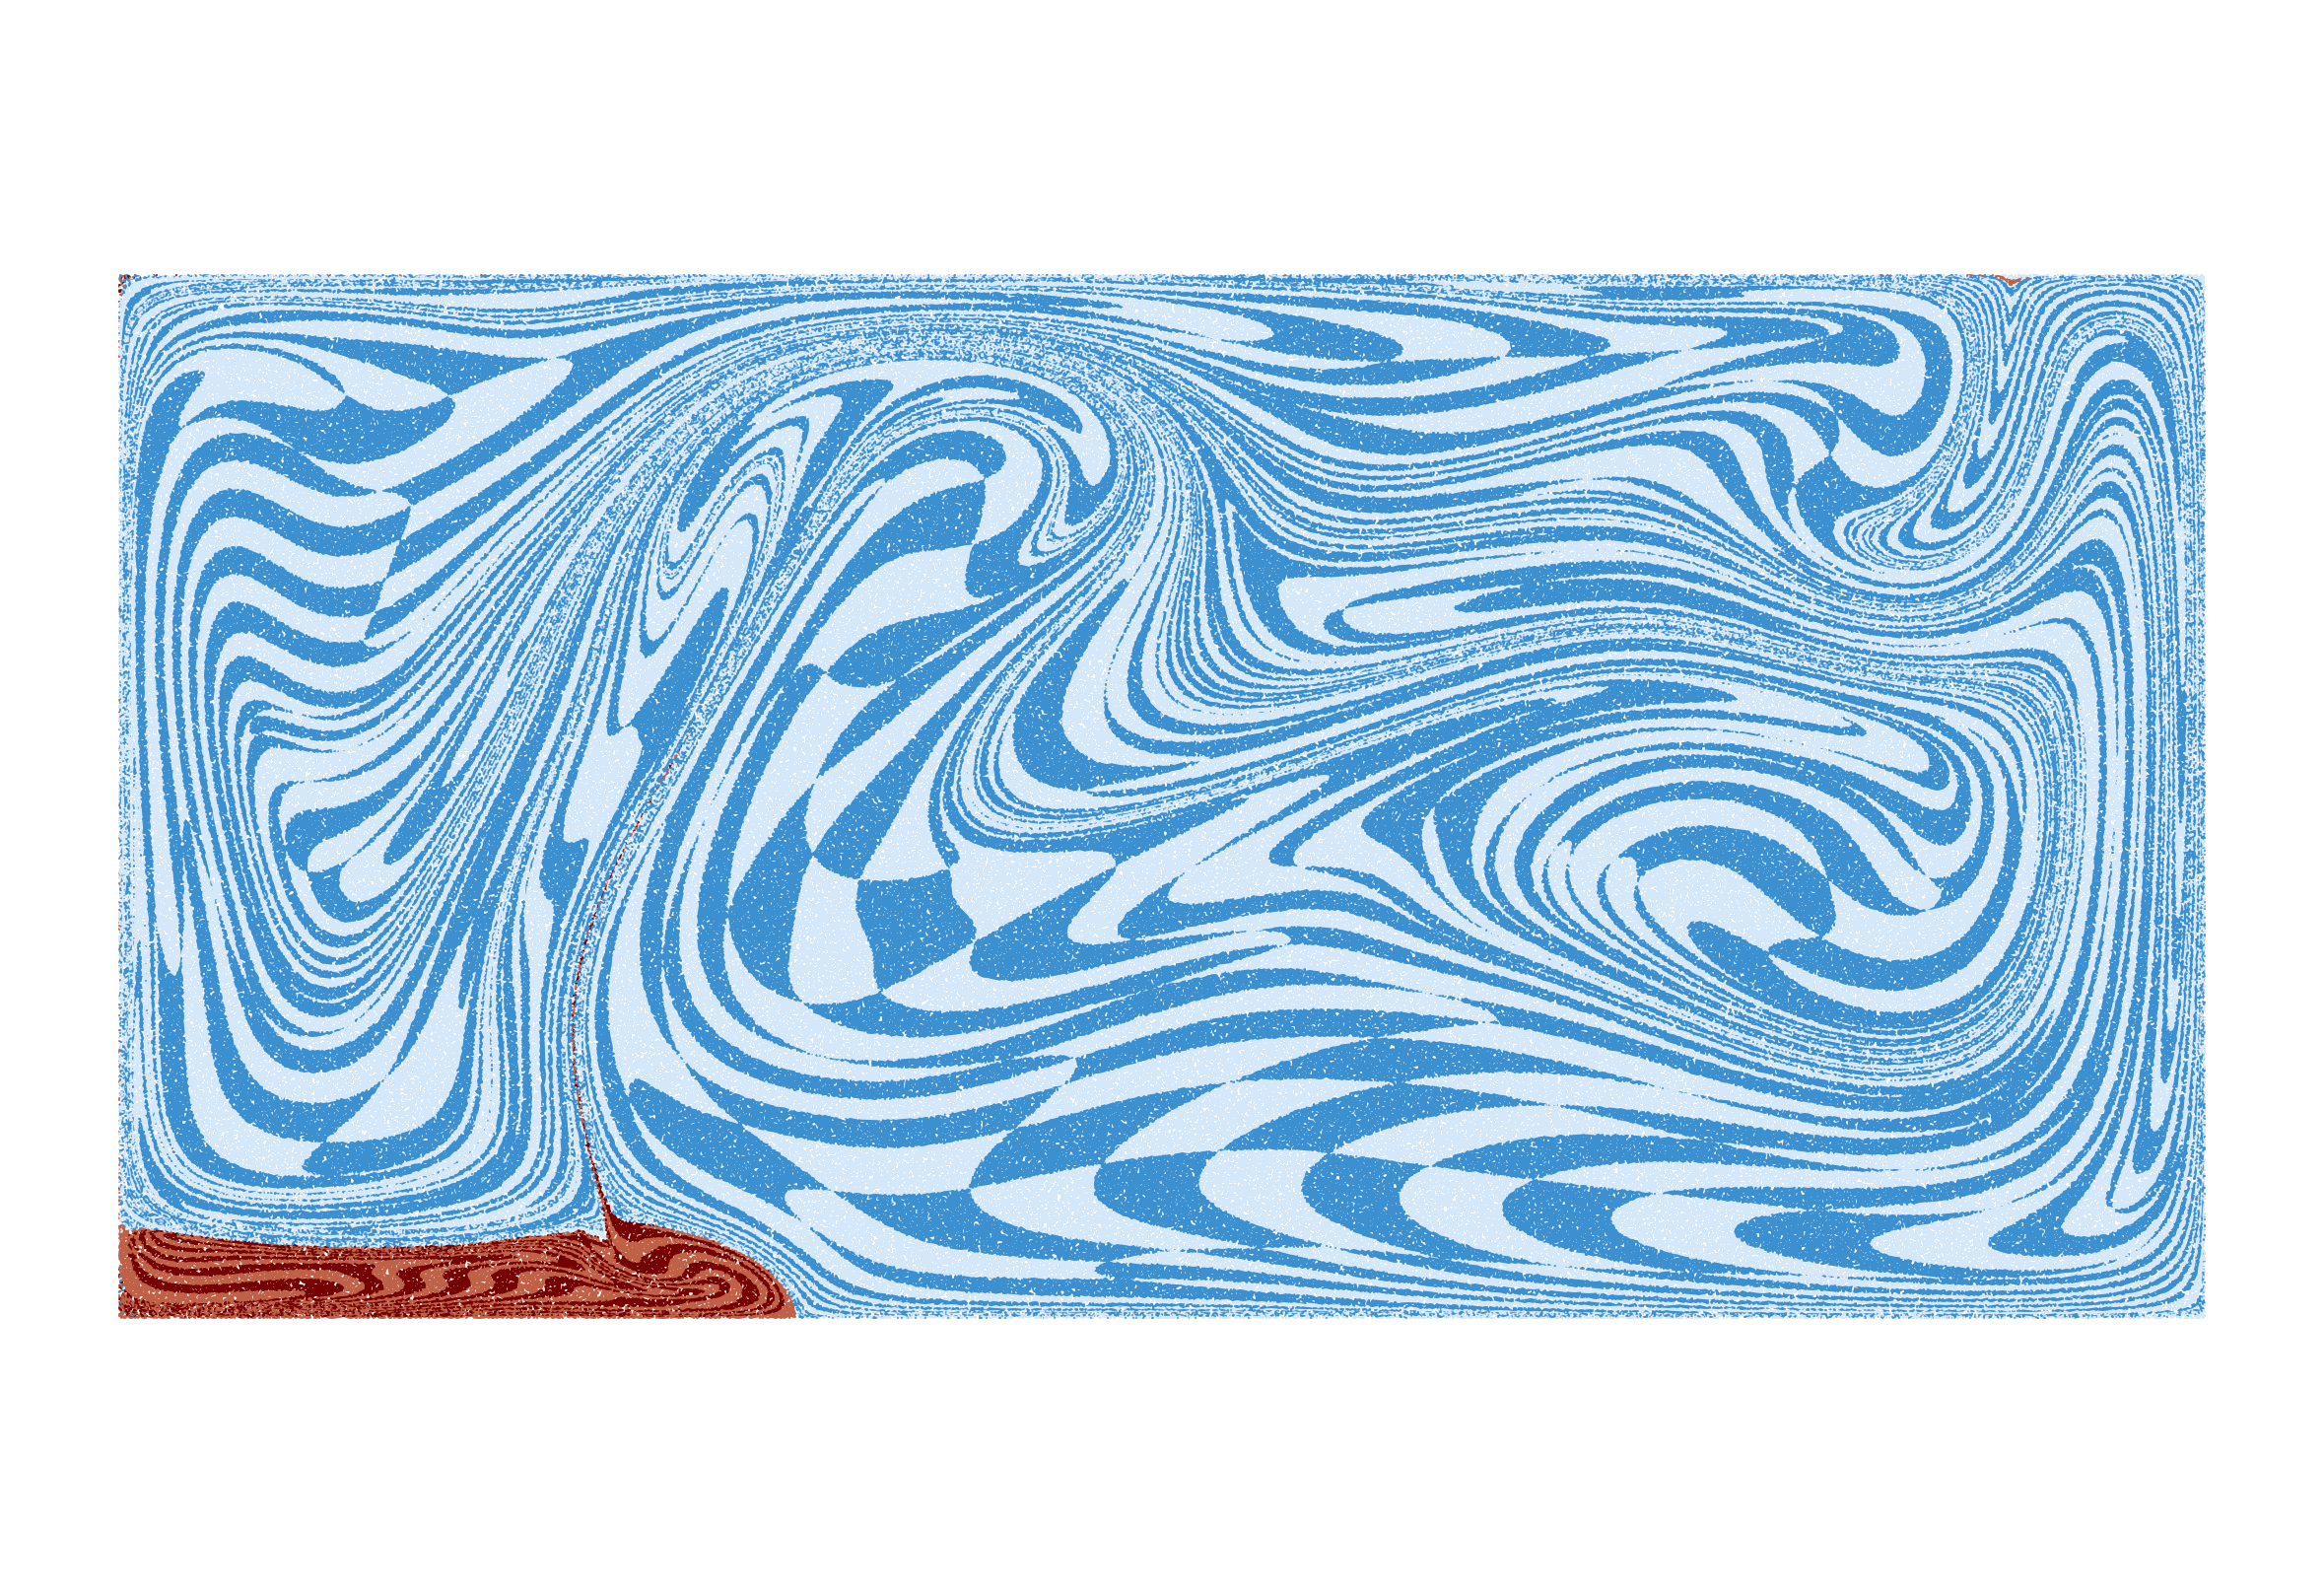
\includegraphics[width=0.23\linewidth]{images/benchmark_thinlayer/maarkers0175}\\
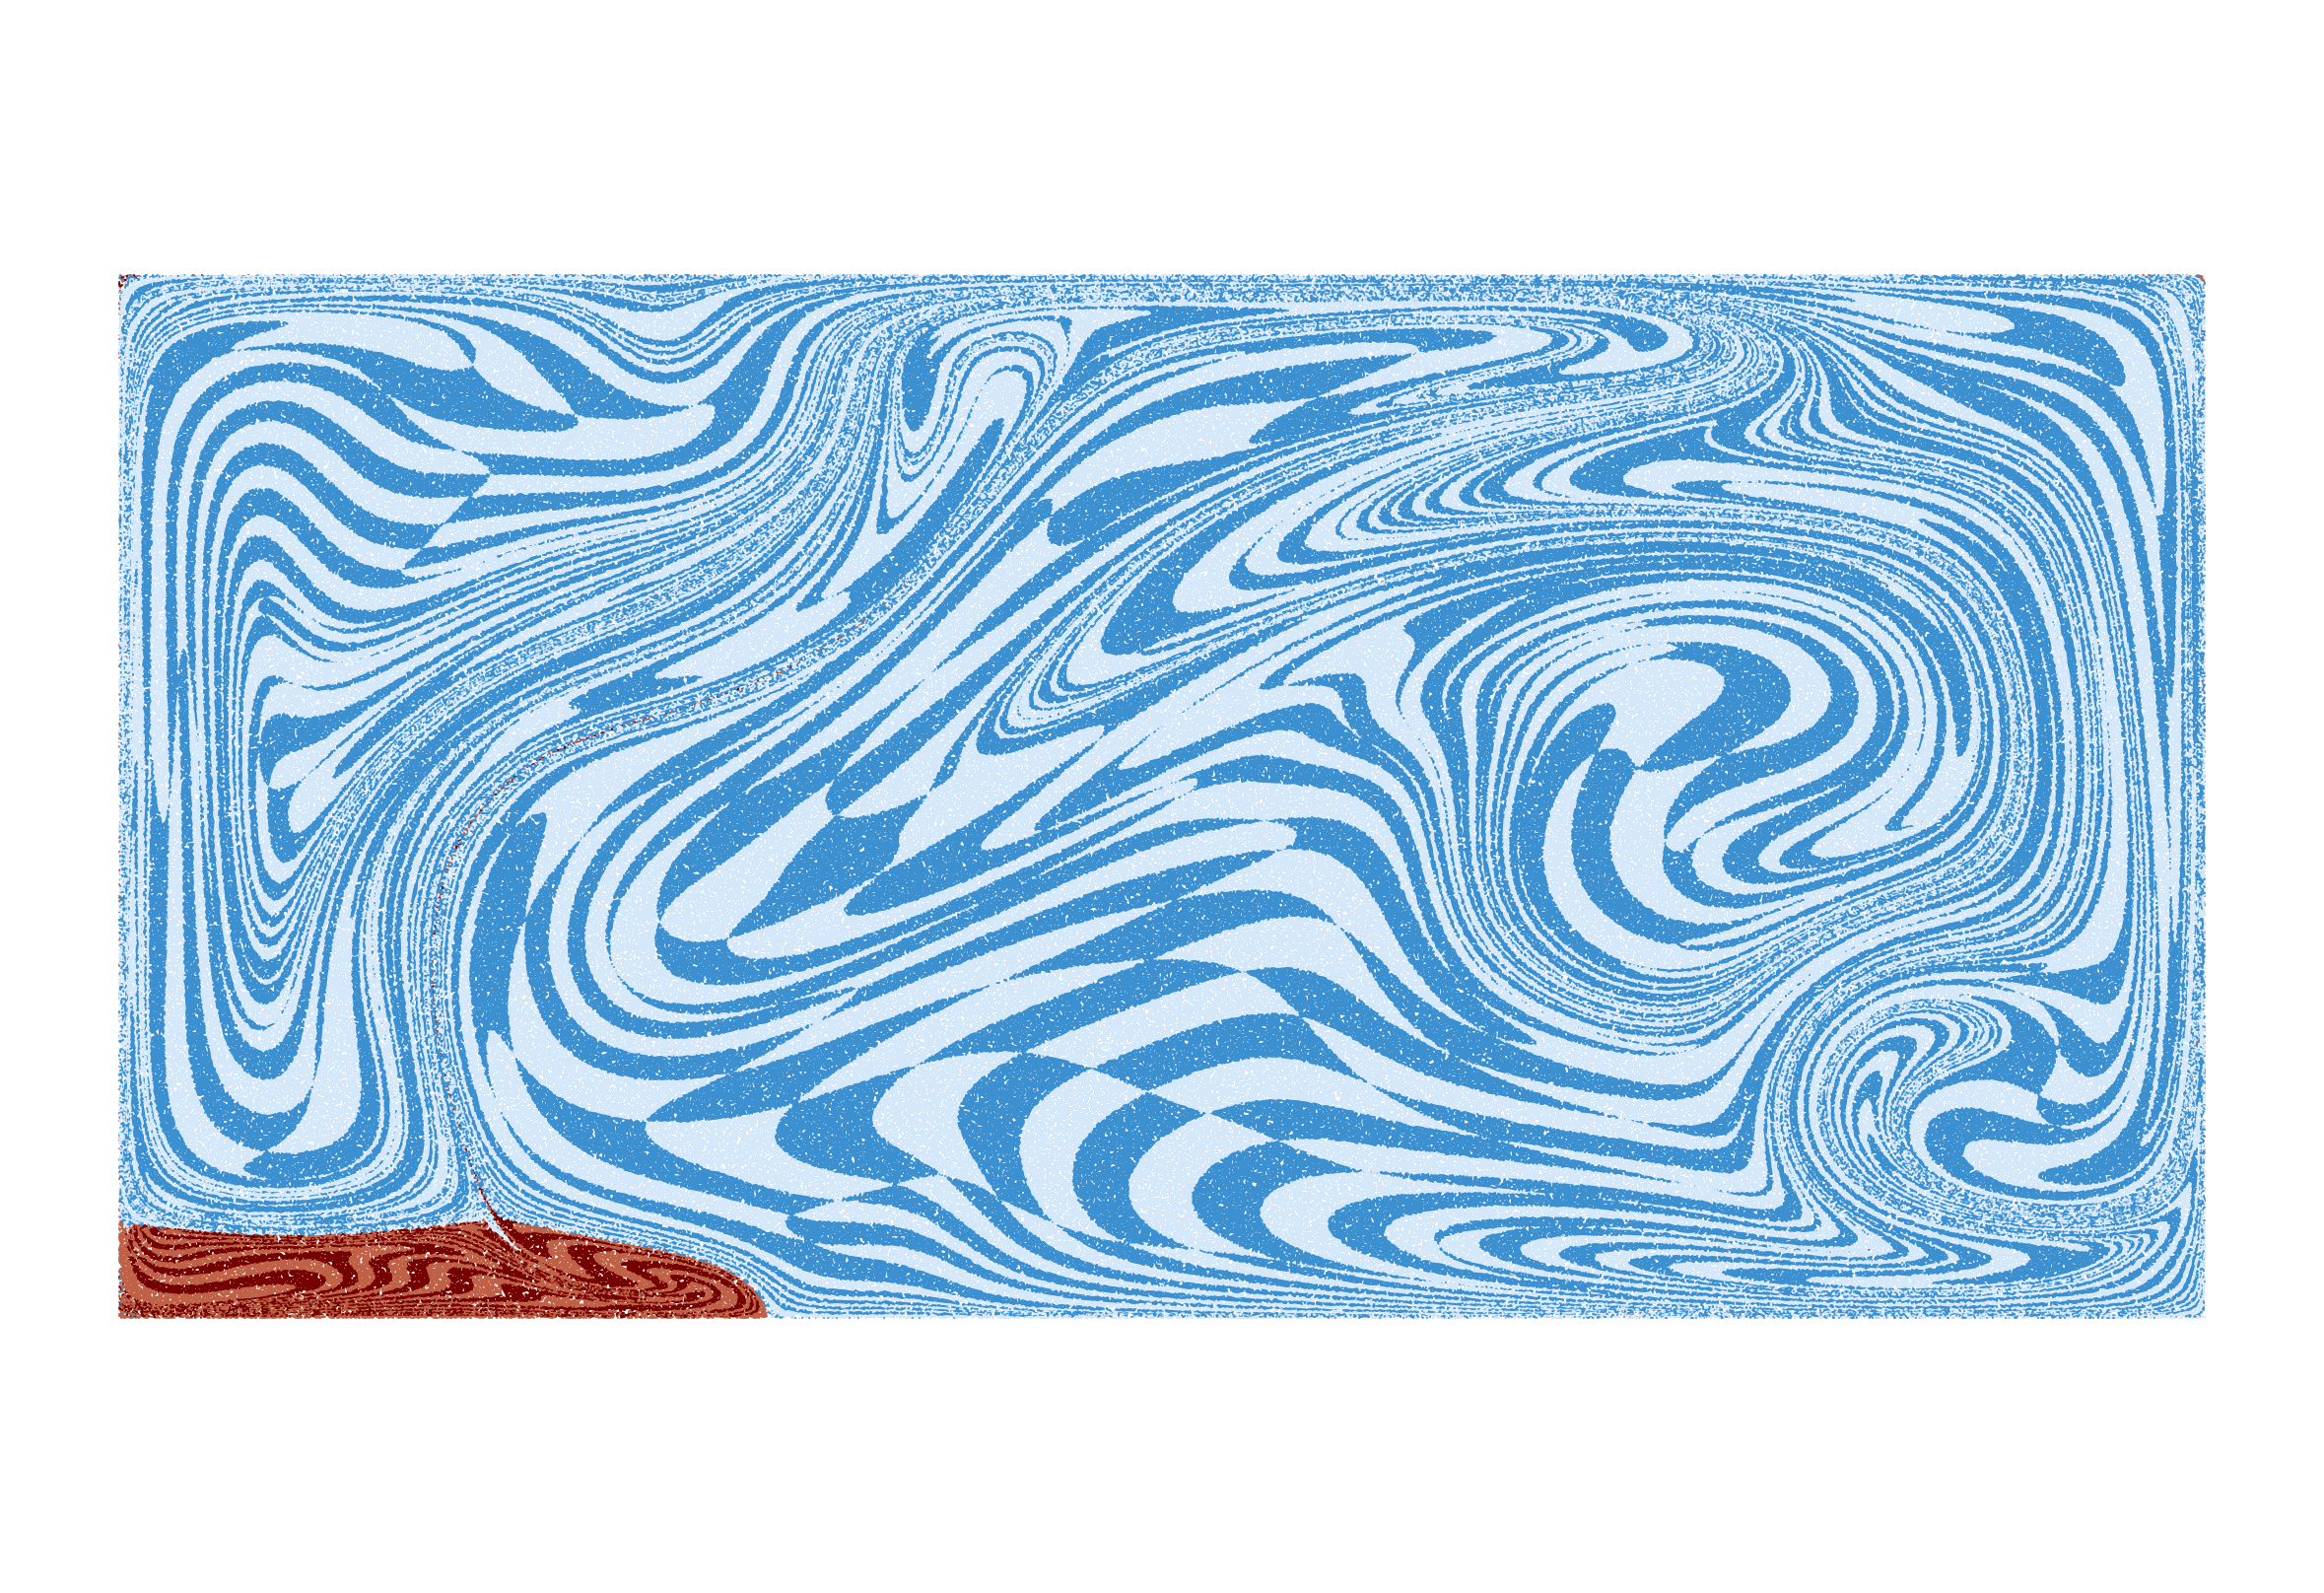
\includegraphics[width=0.23\linewidth]{images/benchmark_thinlayer/maarkers0200}
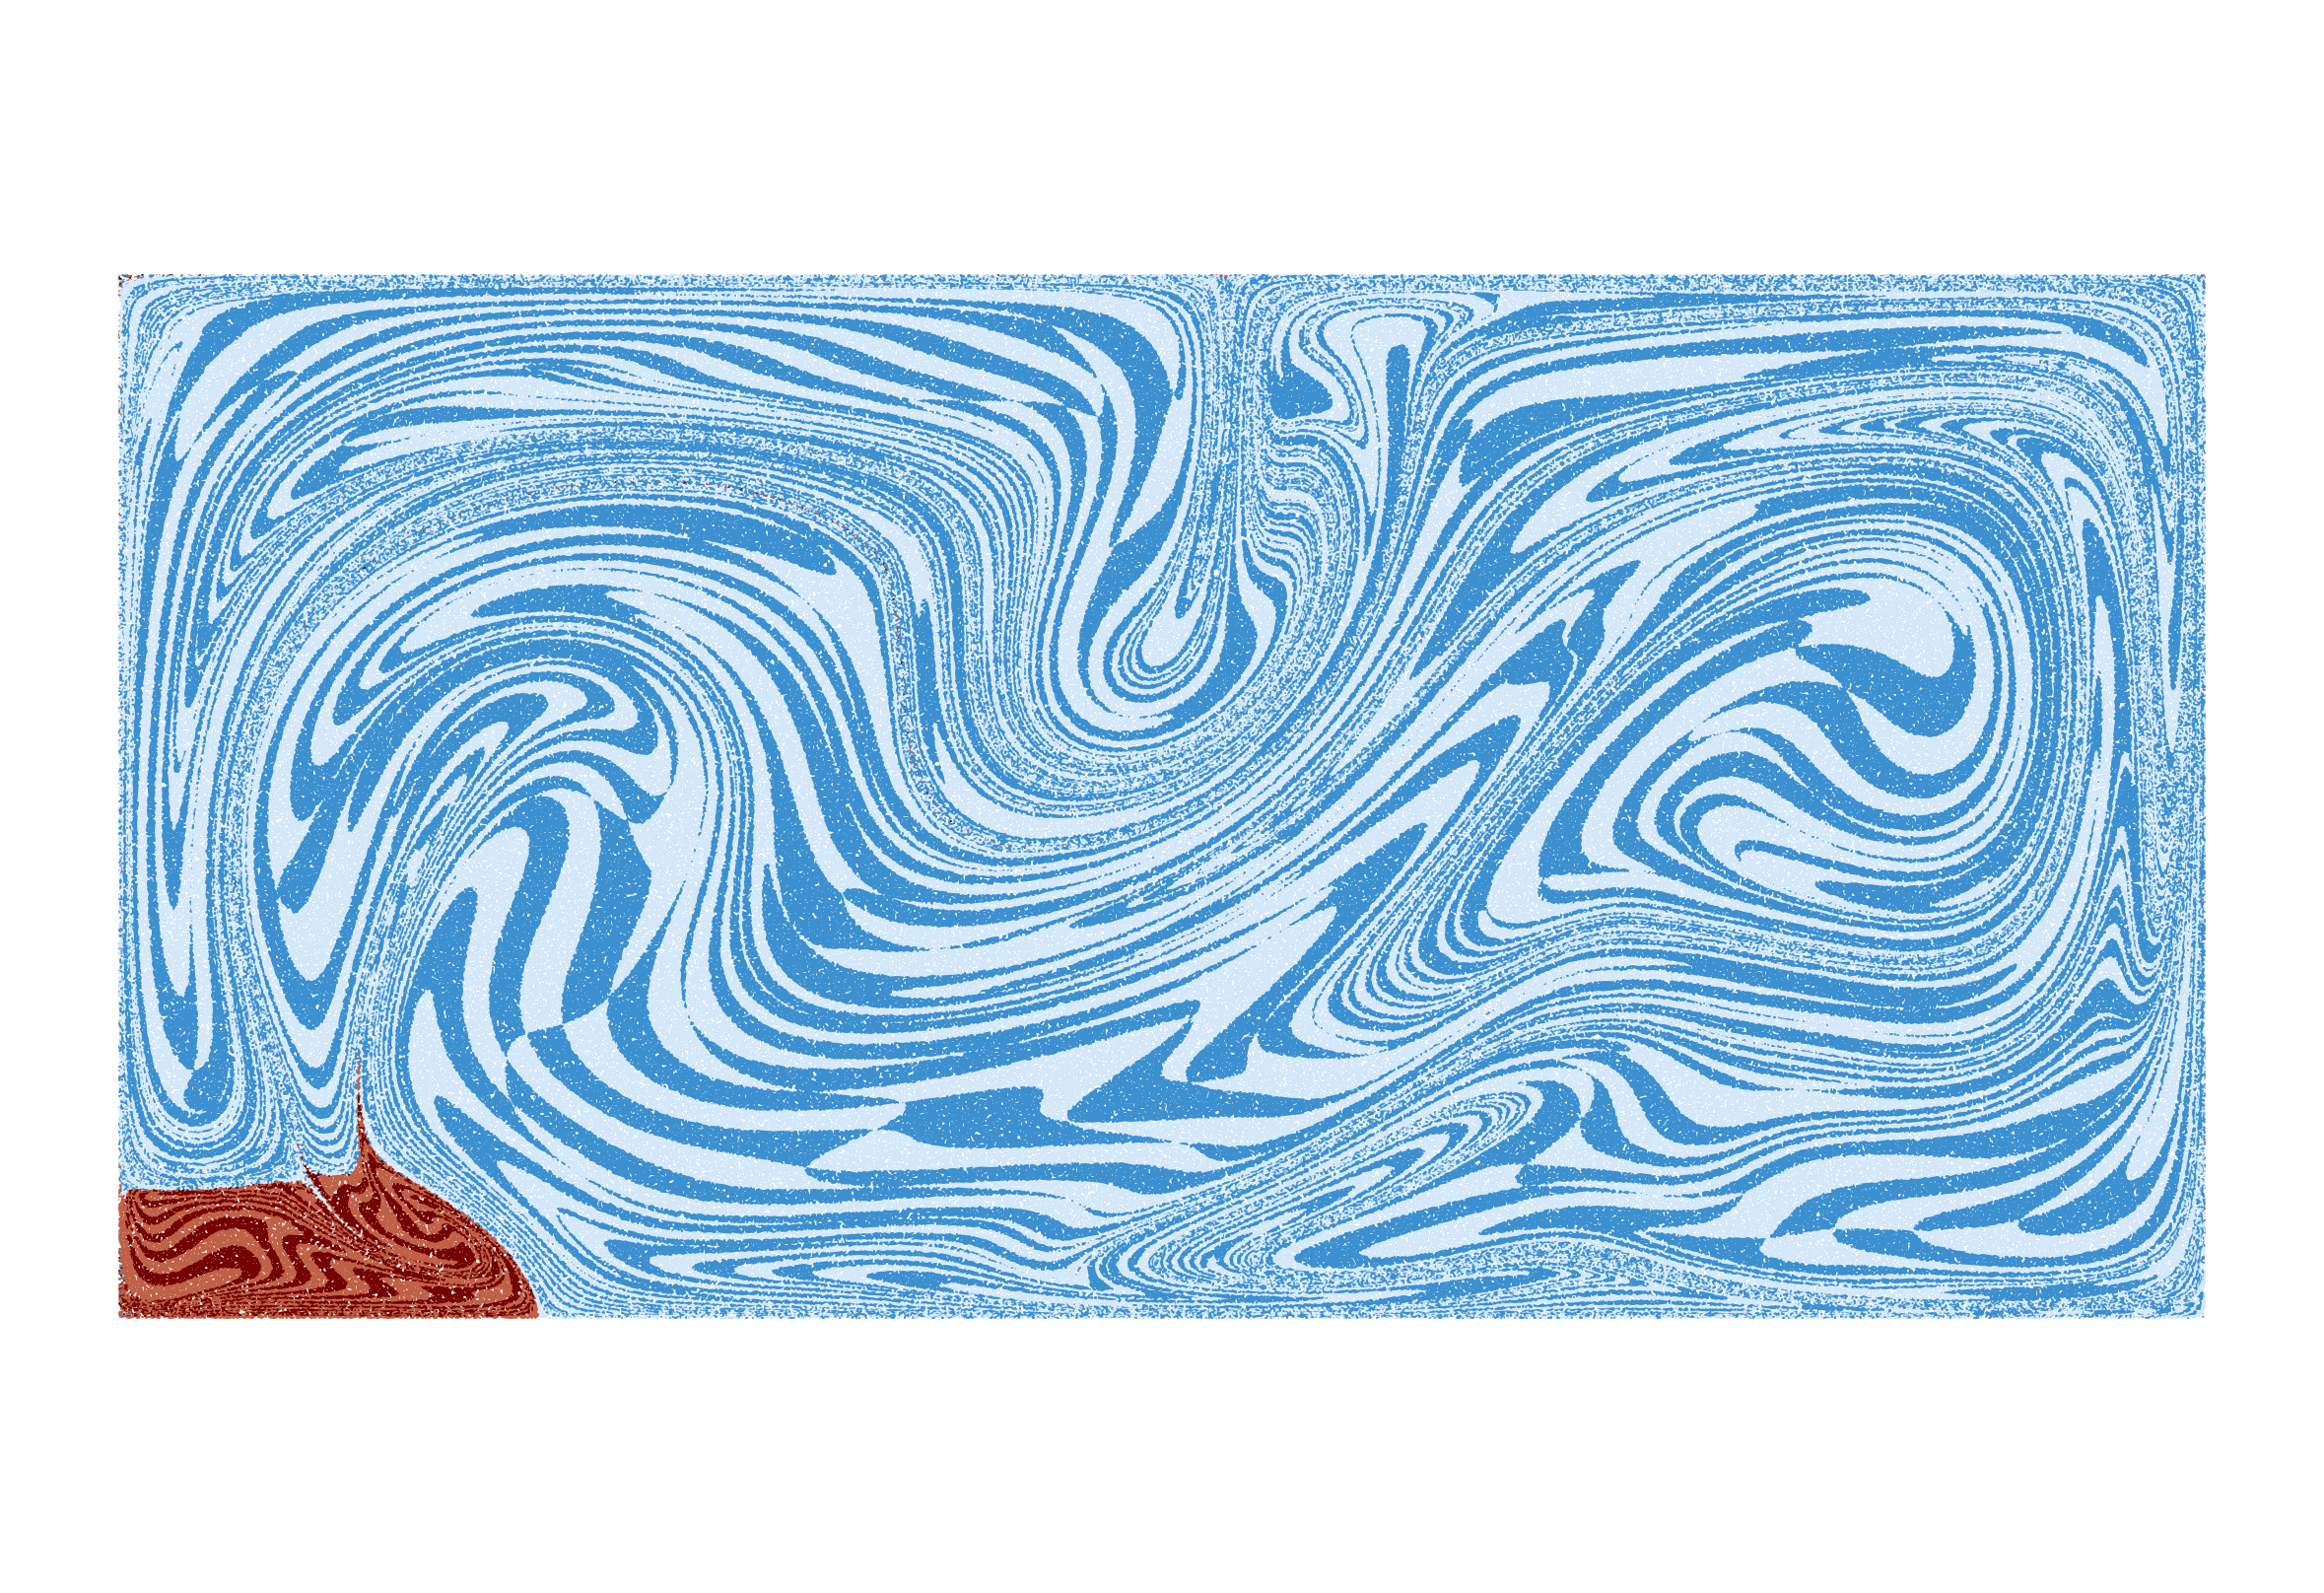
\includegraphics[width=0.23\linewidth]{images/benchmark_thinlayer/maarkers0225}
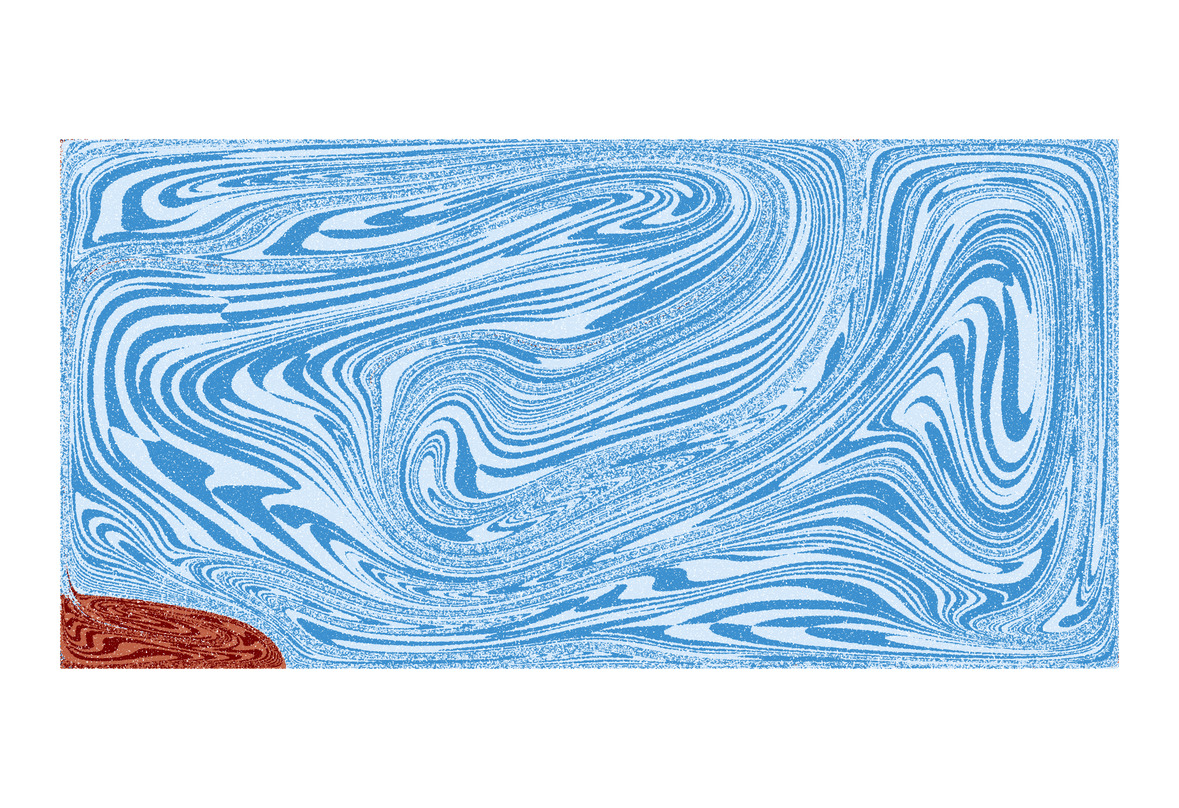
\includegraphics[width=0.23\linewidth]{images/benchmark_thinlayer/maarkers0250}
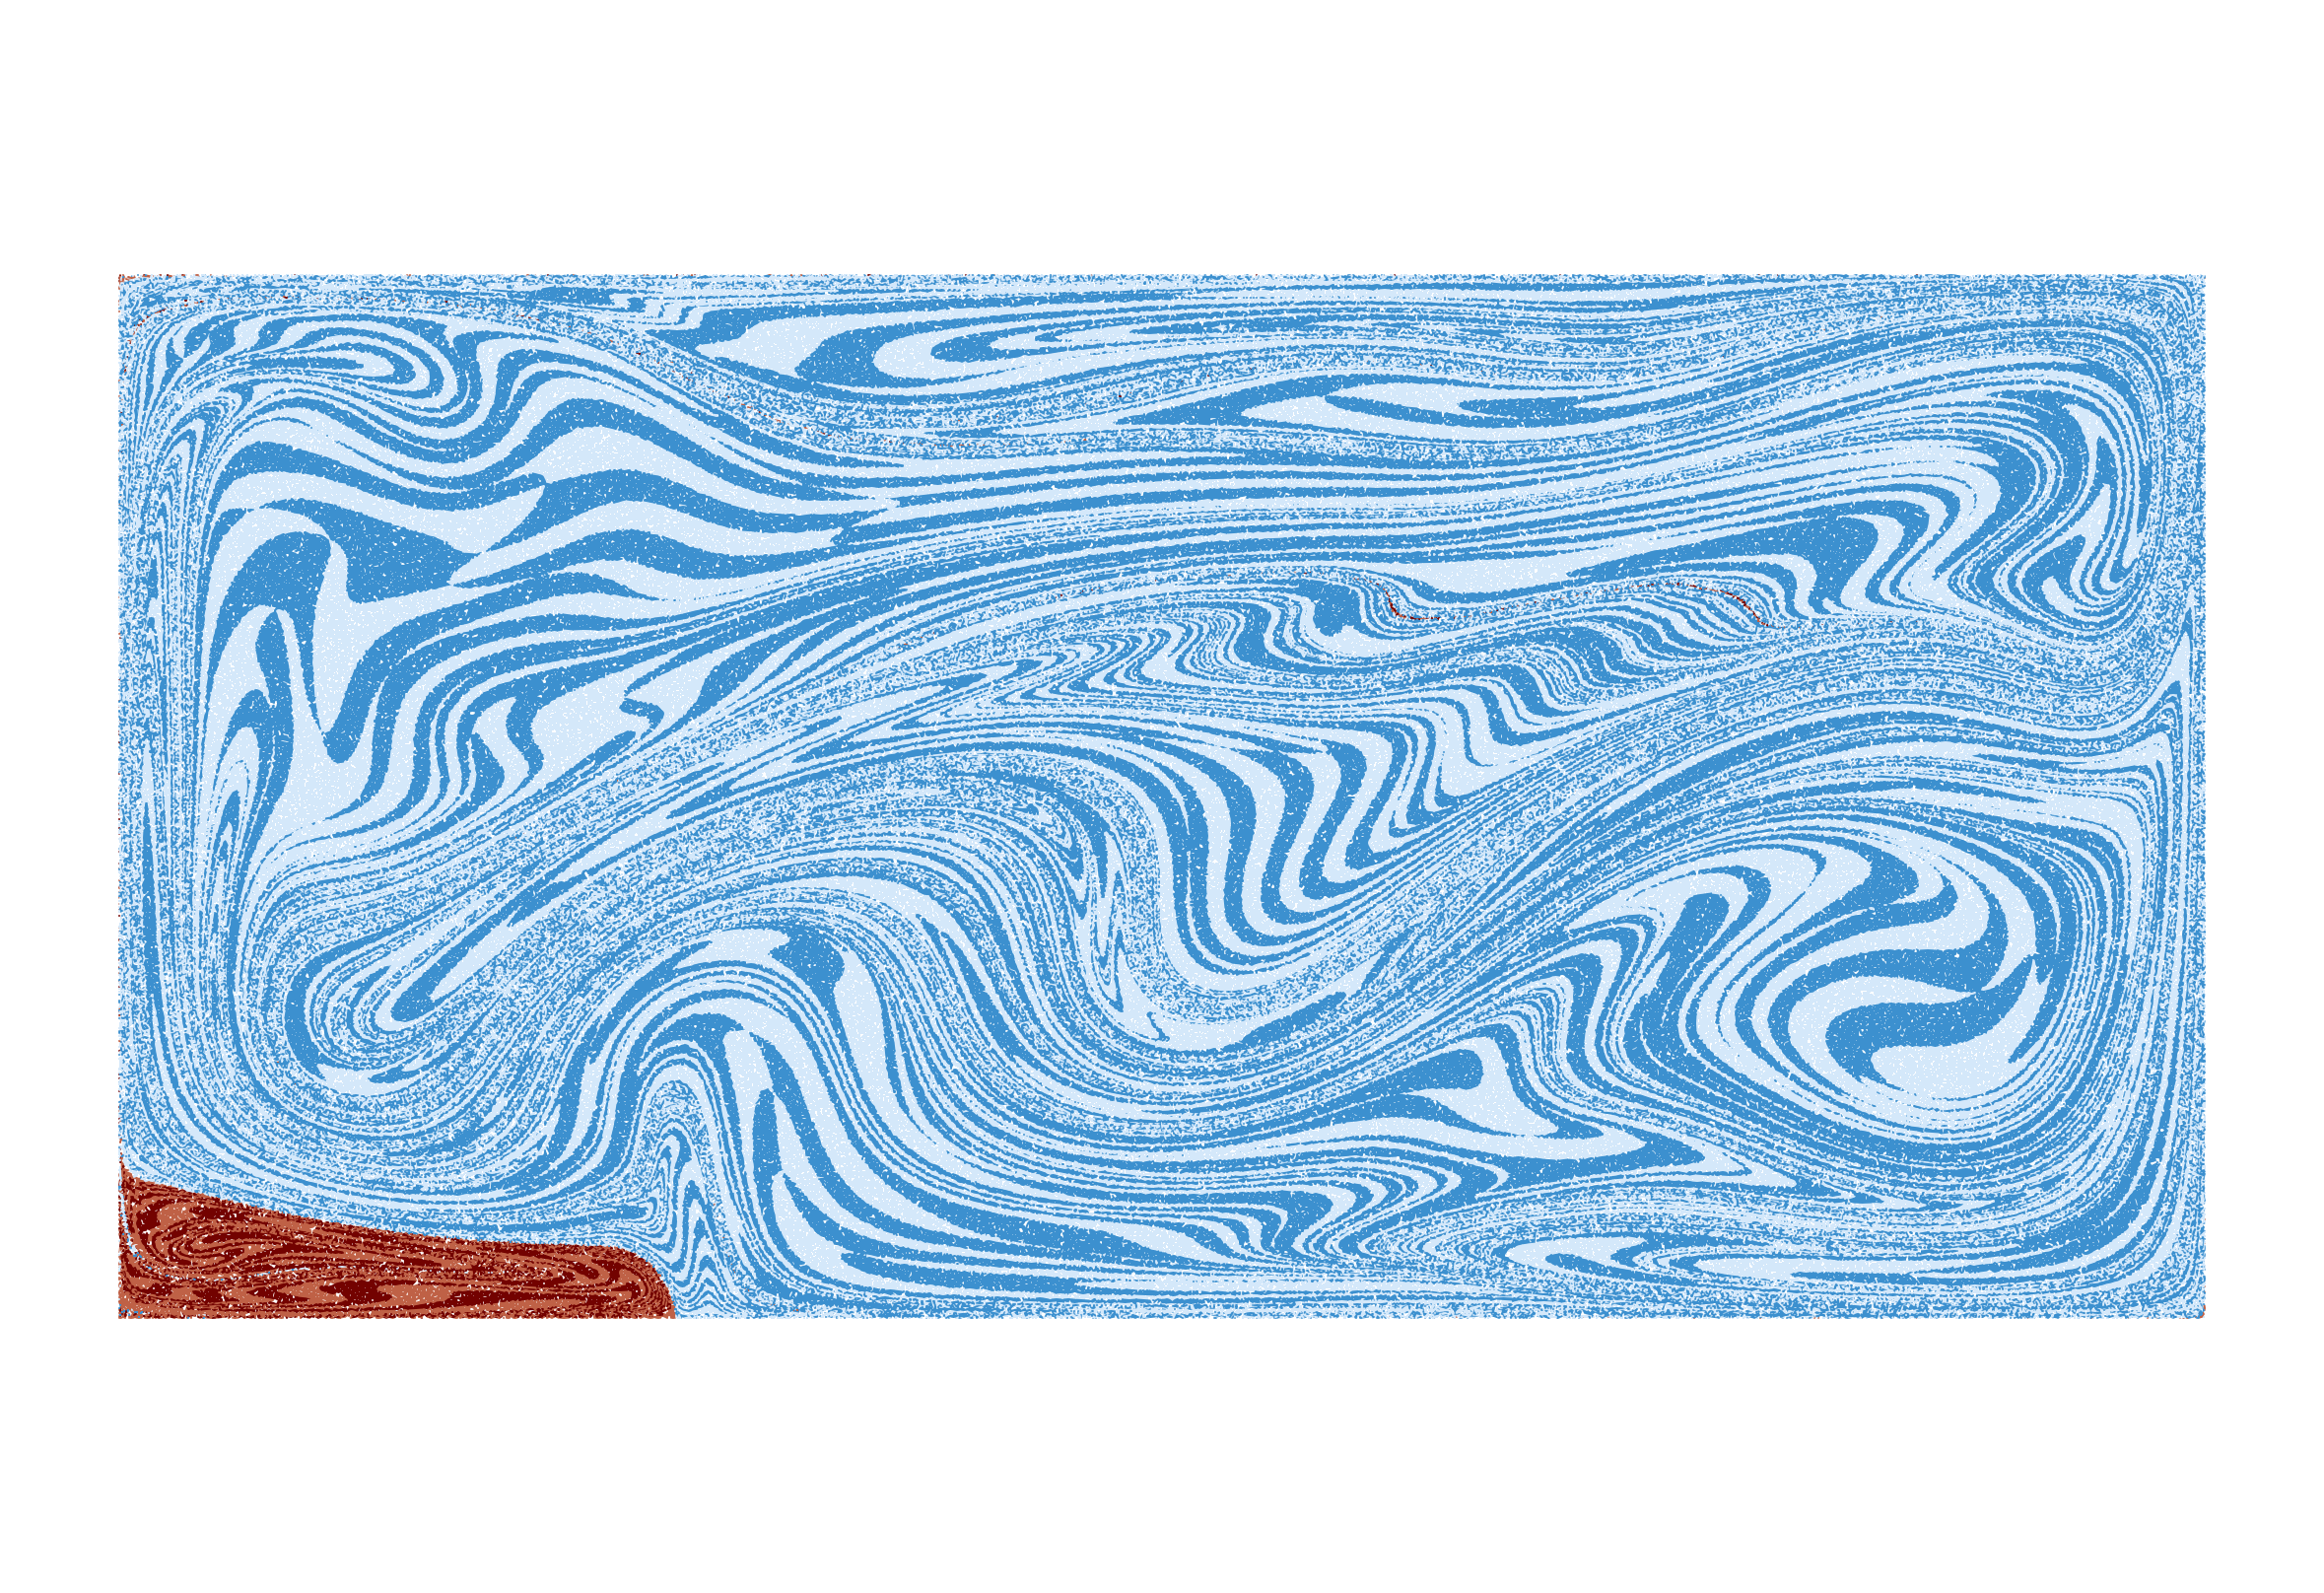
\includegraphics[width=0.23\linewidth]{images/benchmark_thinlayer/maarkers0275}\\
{\scriptsize  marker distribution as obtained with ELEFANT for 
grid 240x120, init\_marker\_density=7, random distribution, 
CFL=0.25, rkmethod=2, m\_to\_q=2. Unpublished.}
\end{center}


